 %%%%%%%%%%%%%%%%%%%% author.tex %%%%%%%%%%%%%%%%%%%%%%%%%%%%%%%%%%%
%
% sample root file for your "contribution" to a contributed volume
%
% Use this file as a template for your own input.
%
%%%%%%%%%%%%%%%% Springer %%%%%%%%%%%%%%%%%%%%%%%%%%%%%%%%%%


% RECOMMENDED %%%%%%%%%%%%%%%%%%%%%%%%%%%%%%%%%%%%%%%%%%%%%%%%%%%
\RequirePackage{amsmath}
\documentclass[graybox]{svmult}

% choose options for [] as required from the list
% in the Reference Guide

\usepackage{amssymb}       % selects Times Roman as basic font
\usepackage{helvet}         % selects Helvetica as sans-serif font
\usepackage{courier}        % selects Courier as typewriter font
\usepackage{type1cm}        % activate if the above 3 fonts are
                            % not available on your system
%
\usepackage{makeidx}         % allows index generation
\usepackage{graphicx}        % standard LaTeX graphics tool
                             % when including figure files
\usepackage{multicol}        % used for the two-column index
\usepackage[bottom]{footmisc}% places footnotes at page bottom

\usepackage{psfrag,bbm,epsf}
\usepackage{xspace,subfigure}
\usepackage{comment}
\usepackage{amssymb, xcolor,enumerate,float,mathtools}
\usepackage{algpseudocode}
\usepackage{algorithm, algorithmicx}
\usepackage[numbers]{natbib}
\usepackage{enumerate,multirow,booktabs}
\usepackage{url}
\usepackage{natbib}
\usepackage{showlabels}

\algnewcommand\algorithmicparam{\textbf{Parameters:}}
\algnewcommand\PARAM{\item[\algorithmicparam]}
\algnewcommand\algorithmicinput{\textbf{Input:}}
\algnewcommand\INPUT{\item[\algorithmicinput]}
\algnewcommand\algorithmicoutput{\textbf{Output:}}
\algnewcommand\OUTPUT{\item[\algorithmicoutput]}
%\algnewcommand\STATE{\item}
\algnewcommand\RETURN{\State \textbf{Return }}

\newcommand{\blind}{1}
\newtheorem{lem}{Lemma}
\newtheorem{thm}{Theorem}
\newtheorem{pro}{Proposition}
\newtheorem{defn}{Definition}
\newtheorem{rmk}{Remark}
\newtheorem{cor}{Corollary}
\newcommand{\reals}{\mathbb{R}}
\newcommand{\naturals}{\mathbb{R}}
\newcommand{\va}{\boldsymbol{a}}
\newcommand{\vb}{\boldsymbol{b}}
\newcommand{\vc}{\boldsymbol{c}}
\newcommand{\vx}{\boldsymbol{x}}
\newcommand{\vX}{\boldsymbol{X}}
\newcommand{\vt}{\boldsymbol{t}}
\newcommand{\vz}{\boldsymbol{z}}
\newcommand{\vu}{\boldsymbol{u}}
\newcommand{\vv}{\boldsymbol{v}}
\newcommand{\vy}{\boldsymbol{y}}
\newcommand{\fraku}{\mathfrak{u}}
\newcommand{\frakv}{\mathfrak{v}}
\newcommand{\mX}{{\mathsf X}}
\newcommand{\vinfty}{\boldsymbol{\infty}}
\newcommand{\vzero}{\boldsymbol{0}}
\newcommand{\vPsi}{\boldsymbol{\Psi}}
\newcommand{\dif}{{\rm d}}
\DeclareMathOperator{\sign}{sign}
\DeclareMathOperator*{\argmax}{argmax}
\newcommand{\Udes}{\mathcal{U}}
\newcommand{\Xdes}{\mathcal{X}}
\newcommand{\FXdes}{F_{\Xdes}}
\newcommand{\cm}{\mathcal{M}}
\newcommand{\ch}{\mathcal{H}}
\newcommand{\MATLAB}{\textsc{Matlab}\xspace}
\newcommand{\Ftar}{F}
\newcommand{\ftar}{\varrho}
\newcommand{\cube}{\ensuremath{(0,1)^d}}
\newcommand{\bbone}{\mathbbm{1}}
\newcommand{\Ex}{\mathbb{E}}
\newcommand{\ip}[3][{}]{\ensuremath{\left \langle #2, #3 \right \rangle_{#1}}}
\newcommand{\norm}[2][{}]{\ensuremath{\left \lVert #2 \right \rVert}_{#1}}
\DeclareMathOperator{\cov}{cov}
\DeclareMathOperator{\err}{err}
\newcommand{\unif}{\textup{unif}}
\newcommand{\normal}{\textup{normal}}
\newcommand{\frakd}{\mathfrak{d}}
\newcommand{\tK}{\widetilde{K}}
\newcommand{\tOmega}{\widetilde{\Omega}}
\newcommand{\tvarrho}{\widetilde{\varrho}}
\newcommand{\Order}{\mathcal{O}}

\def\abs#1{\ensuremath{\left \lvert #1 \right \rvert}}

\usepackage{bm} %to get bold math fonts

\newcommand{\FJH}[1]{{\color{blue}Fred: #1}}
\newcommand{\LK}[1]{{\color{green}Lulu: #1}} %choose your color
\newcommand{\YL}[1]{{\color{teal}Yiou: #1}} %choose your color




% see the list of further useful packages
% in the Reference Guide

\makeindex             % used for the subject index
                       % please use the style svind.ist with
                       % your makeindex program

%%%%%%%%%%%%%%%%%%%%%%%%%%%%%%%%%%%%%%%%%%%%%%%%%%%%%%%%%%%%%%%%%%%%%%%%%%%%%%%%%%%%%%%%%

\begin{document}

\title*{Are Transformed Low Discrepancy Points Also Low Discrepancy?}
% Use \titlerunning{Short Title} for an abbreviated version of
% your contribution title if the original one is too long
\author{Yiou Li, Lulu Kang, and Fred Hickernell}
% Use \authorrunning{Short Title} for an abbreviated version of
% your contribution title if the original one is too long
\institute{Yiou Li \at DePaul University, 2320 N. Kenmore Avenue, Chicago, IL 60614 \email{yli139@depaul.edu}
\and Lulu Kang \at Illinois Institute of Technology, 10 W 32nd Street, Chicago, IL 60616 \email{lkang2@iit.edu} 
\and 
Fred Hickernell \at Illinois Institute of Technology, 10 W 32nd Street, Chicago, IL 60616 \email{hickernell@iit.edu}}
%
% Use the package "url.sty" to avoid
% problems with special characters
% used in your e-mail or web address
%
\maketitle

\abstract{Write me later}

\section{Introduction}

Professor Kai-Tai Fang and his collaborators have demonstrated the effectiveness of low discrepancy points as space filling designs \cite{FanWan94, FanLiSud06, FangHic07a}.  
They promoted discrepancy as a quality measure for statistical experimental designs to the statistics, science, and engineering communities \cite{FanMaWin02, FanMuk00, FanMa01a, FanMa01b}. 

Low discrepancy designs, $\Udes = \{\vu_i\}_{i=1}^N$, are typically constructed so that their empirical distribution, $F_\Udes$, approximates $F_\unif$, the uniform distribution on the unit cube, \cube.  
The discrepancy measures how large $F_\unif-F_\Udes$ is.  

When the target distribution for the design, $\Ftar$, defined over the experimental domain $\Omega$, is \emph{not} the uniform distribution on the unit cube, then one typically constructs the desired design, $\Xdes$, by transforming a low discrepancy uniform design, i.e., 
\begin{equation} \label{eq:transPts}
\Xdes = \{\vx_i\}_{i=1}^N = \{\vPsi(\vu_i)\}_{i=1}^N = \vPsi(\Udes), \qquad \vPsi: \cube \to \Omega.
\end{equation}
Note that $\Ftar$ may differ from $F_\unif$ because $\Omega \ne \cube$ and/or $\Ftar$ is non-uniform.  
A natural transformation, $\vPsi(\vu)=[\Psi_1(u_1),\ldots,\Psi_d(u_d)]$, when $\Ftar$ has independent marginals, is the inverse distribution transformation:
\begin{equation}\label{eq:inverse}
\Psi_j(u_j) = F_j^{-1}(u_j), \quad j =1, \ldots, d, \qquad \text{where } \Ftar(\vx) = F_1(u_1) \cdots F_d(u_d).
\end{equation}
A number of transformation methods for different distributions can be found in \cite{devroye2006nonuniform} and Professor Fang's book \cite{FanWan94}.

The question addressed in this chapter is whether the design $\Xdes$ resulting from transformation \eqref{eq:transPts} of a low discrepancy design, $\Udes$, is itself low discrepancy with respect to the target distribution $\Ftar$. 
In other words, 
\begin{equation} \label{BigQ} \tag{Q}
\text{\emph{does small $F_\unif - F_\Udes$ imply small $\Ftar - F_\Xdes$?}}
\end{equation}
We demonstrate that the answer may be yes or no, depending on how the question is posed.  
We discuss both cases.  
For illustrative purposes, we consider the case where $\Ftar$ is the multivariate standard normal distribution.

In the rest of this chapter, we first explain the discrepancy that measures how large $\Ftar - F_\Xdes$ is and motivate it from three different perspectives.  Next, we show how the inverse transformation can lead to does not always preserve the low discrepancy of a design.
We also propose a remedy method to improve the design in terms of the discrepancy between $\Ftar$ and $F_\Xdes$. 
Numerical examples are used to show the performance of the method. 

%%%%%%%%%%%%%%%%%%%%%%%%%%%%%%%%%%%%%%%%%%%%%%%%%%%%%%%%%%%%%%%%%%%%%%%
%%%%%%%%%%%%%%%%%%%%%%%%%%%%%%%%%%%%%%%%%%%%%%%%%%%%%%%%%%%%%%%%%%%%%%%
\section{The Discrepancy}
%%%%%%%%%%%%%%%%%%%%%%%%%%%%%%%%%%%%%%%%%%%%%%%%%%%%%%%%%%%%%%%%%%%%%%%
%%%%%%%%%%%%%%%%%%%%%%%%%%%%%%%%%%%%%%%%%%%%%%%%%%%%%%%%%%%%%%%%%%%%%%%

Experimental design theory based on  discrepancy assumes an experimental region, $\Omega$, and a target probability distribution, $\Ftar:\Omega \to [0,1]$, which is known a priori. We assume that $\Ftar$ has a probability density, $\ftar$.  It is convenient to also work with measures, $\nu$, defined on $\Omega$.  If $\nu$ is a probability measure, the associated probability distribution is given by $F(\vx) = \nu((-\vinfty,\vx])$.  The Dirac measure, $\delta_{\vx}$ is the probability measure assigning unit measure to the point $\vx$.  A design, $\Xdes = \{\vx_i\}_{i=1}^N$, is a finite set of points that has an associated empirical distribution, $F_{\Xdes}  = N^{-1} \sum_{i=1}^N \bbone_{(-\vinfty,\vx_i]}$ as well as an associated empirical measure, $\nu_{\Xdes}  = N^{-1} \sum_{i=1}^N \delta_{\vx_i}$.

Our notation for discrepancy takes the form of 
\[
 D(F_{\Xdes},F,K), \ D(\Xdes,F,K), \ D(\Xdes,\varrho,K), \ D(\Xdes,\nu,K), \ D(\nu_{\Xdes},\nu,K), \text{ etc.}, 
\]
all of which mean the same thing.  The first argument always refers to the design, the second argument always refers to the target, and the third argument is a symmetric, positive definite kernel, which is explained below.  We abuse the discrepancy notation because sometimes it is convenient to refer to the design as a set, $\Xdes$, other times by its empirical distribution, $F_{\Xdes}$, and other times by its empirical measure, $\nu_{\Xdes}$.  Likewise, sometimes it is convenient to refer the target as a probability measure,  $\nu$, other times by its distribution function, $F$, and other times by its density function, $\varrho$.

In the remainder of this section we provide three interpretations of the discrepancy, summarized in Table \ref{tab:ThreeInterpTable}.  These results are derived previously in various places, including \cite{Hic99a}.  One interpretation is the norm of $\nu - \nu_{\Xdes}$.  The second and third interpretations consider the problem of evaluating the mean of a random variable $Y=f(\vX)$, or equivalently a multidimensional integral
\begin{equation}\label{eq:integration}
\mu = \Ex(Y) = \Ex[f(\vX)] = \int_{\Omega} f(\vx) \, \varrho(\vx) \, \dif \vx,
\end{equation}
where $\vX$ is a random vector with density $\varrho$. The second
interpretation is worst-case cubature error for integrands, $f$, in the unit ball of a Hilbert space.  The third interpretation is the root mean squared cubature error for integrands, $f$ which are realizations of a stochastic processes.

\begin{table}
\centering
\caption{Three interpretations of the discrepancy}
\vspace{-3ex}
\begin{equation*}
\begin{array}{c@{\qquad}ccc}
\text{Kernel Interpretation} & \text{Discrepancy } D(\Xdes,\nu,K) = D(\Xdes,\varrho,K)\\
\toprule \\[-1ex]
K(\vt,\vx) = \ip[\cm]{\delta_{\vt}}{\delta_{\vx}} & \norm[\cm]{\nu - \nu_{\Xdes}} \\[2ex]
f(\vx) = \ip[\ch]{K(\cdot,\vx)}{f} & \displaystyle \sup_{f \in \ch : \norm[\ch]{f} \le 1} \abs{\int_{\Omega} f(\vx) \, \varrho(\vx) \, \dif \vx - \frac 1N \sum_{i=1}^N f(\vx_i)}\\[4ex]
K(\vt,\vx) = \cov\bigl(f(\vt), f(\vx) \bigr) & \displaystyle \sqrt{\Ex \abs{\int_{\Omega} f(\vx) \, \varrho(\vx) \, \dif \vx - \frac 1N \sum_{i=1}^N f(\vx_i)}^2}\\\bottomrule
\end{array}
\end{equation*}
\label{tab:ThreeInterpTable}
\end{table}

%%%%%%%%%%%%%%%%%%%%%%%%%%%%%%%%%%%%%%%%%%%%%%%%%%%%%%%%%%%%%%%%%%%%%%%
\subsection{Definition in Terms of a Norm on a Hilbert Space of Measures}
\label{sec:HilbertMeasures}
%%%%%%%%%%%%%%%%%%%%%%%%%%%%%%%%%%%%%%%%%%%%%%%%%%%%%%%%%%%%%%%%%%%%%%%

Let $(\cm, \ip[\cm]{\cdot}{\cdot})$ be a Hilbert space of measures defined on the experimental region, $\Omega$.  Assume that $\cm$ includes all Dirac measures.  Define the function $K:\Omega \times \Omega \to \reals$ in terms of inner products of Dirac measures:
\begin{equation} \label{kerDeltaDef}
    K(\vt,\vx) := \ip[\cm]{\delta_{\vt}}{\delta_{\vx}}, \qquad \forall \vt, \vx \in \Omega.
\end{equation}
The squared distance between two Dirac measures in $\cm$ is then
\begin{equation} \label{distDelta}
   \norm[\cm]{\delta_{\vx} - \delta_{\vt}}^2 = K(\vt,\vt) - 2K(\vt,\vx) + K(\vx,\vx), \qquad \forall \vt, \vx \in \Omega.
\end{equation}


It is straightforward to show that $ K$ is symmetric in its arguments and positive-definite, namely:
\begin{subequations} \label{eq:sympd}
\begin{gather}
K(\vx, \vt) = K(\vt, \vx) \qquad \forall \vt, \vx\in \Omega,\\
\sum\limits_{i, k=1}^N c_i c_k  K(\vx_i,\vx_k) > 0, \qquad \forall N\in\mathbb{N}, \  \vc \in\mathbb{R}^N, \ \vc \ne \vzero,  \ \Xdes \subset \Omega.
\end{gather}
\end{subequations}
The inner product of arbitrary measures $\lambda, \nu \in \cm$ can be expressed in terms of a double integral of the kernel, $K$:
\begin{equation} \label{ipMdef}
    \ip[\cm]{\lambda}{\nu} = \int_{\Omega \times \Omega} K(\vt,\vx) \, \lambda(\dif \vt) \nu(\dif \vx).
\end{equation}
This can be established directly from \eqref{kerDeltaDef} for $\cm_0$, the vector space spanned by all Dirac measures.  Letting $\cm$ be the closure of the pre-Hilbert space $\cm_0$ then yields \eqref{ipMdef}.

The discrepancy of the design $\Xdes$ with respect to the target probability measure $\nu$ using the kernel $K$ can be defined as the norm of the difference between the target probability measure, $\nu$, and the empirical probability measure for $\Xdes$:
\begin{subequations} \label{eq:discDef}
\begin{align} 
    D^2(\Xdes,\nu,K) & := \norm[\cm]{\nu - \nu_{\Xdes}}^2 \\
    \nonumber
    & = \int_{\Omega \times \Omega} K(\vt,\vx) \, (\nu - \nu_{\Xdes})(\dif \vt) (\nu - \nu_{\Xdes})(\dif \vx) \\
    \nonumber
    & = \int_{\Omega \times \Omega} K(\vt,\vx) \, \nu(\dif \vt) \nu (\dif \vx) - \frac 2N \sum_{i=1}^N \int_{\Omega} K(\vt,\vx_i) \, \nu(\dif \vt)\\
    & \qquad \qquad  + \frac{1}{N^2} \sum_{i,k=1}^N K(\vx_i,\vx_k).
\end{align}
The formula for the discrepancy may be written equivalently in terms of the probability distribution, $F$,  or the probability density, $\varrho$, corresponding to the target probability measure, $\nu$:
\begin{align}
\nonumber
    D^2(\Xdes,F,K)  & = \int_{\Omega \times \Omega} K(\vt,\vx) \, \dif F( \vt) \dif F(\vx) - \frac 2N \sum_{i=1}^N \int_{\Omega} K(\vt,\vx_i)  \, \dif F(\vt) \\ &\qquad \qquad  + \frac{1}{N^2}  \sum_{i,k=1}^N K(\vx_i,\vx_k), \\
\nonumber
   & = \int_{\Omega \times \Omega} K(\vt,\vx) \, \varrho(\vt) \varrho (\vx) \, \dif \vt\dif \vx - \frac 2N \sum_{i=1}^N \int_{\Omega} K(\vt,\vx_i)  \, \varrho(\vt) \, \dif \vt \\
    & \qquad \qquad + \frac{1}{N^2}  \sum_{i,k=1}^N K(\vx_i,\vx_k).
\end{align}
\end{subequations}

The formulas for the discrepancy in \eqref{eq:discDef} depend inherently on the choice of $K$.  That is key to answering our question \eqref{BigQ}.  An often used kernel is 
\begin{equation} \label{eq:OrigKernel}
     K(\vt,\vx)  = \prod\limits_{j=1}^d\left[1+ \frac 12 \left(|t_j|+ |x_j|- |x_j-t_j| \right)\right].
\end{equation}
This kernel is plotted in Figure \ref{fig:kernelpict} for $d=1$.  Note that for this kernel in one dimension the distance between two Dirac measures by \eqref{distDelta} is 
\begin{equation*}
    \norm[\cm]{\delta_{x} - \delta_{t}} = \sqrt{\abs{x-t}}.
\end{equation*}

\begin{figure}
    \centering
    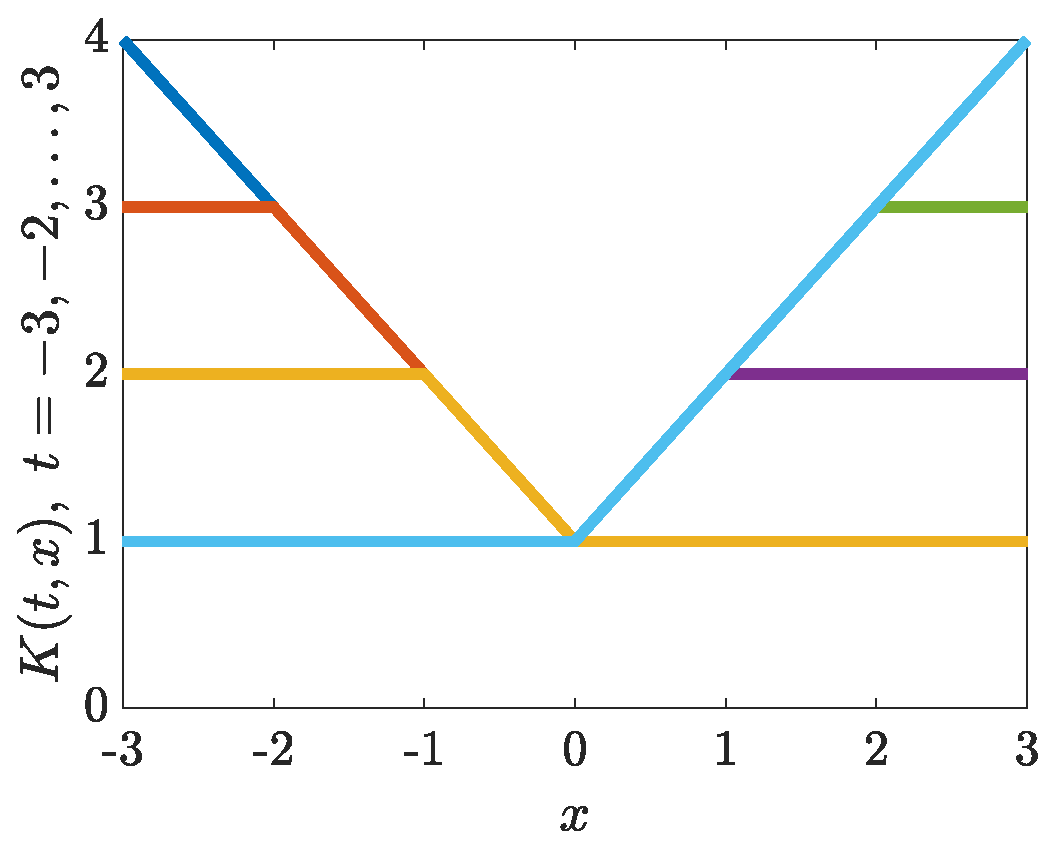
\includegraphics[height = 4cm]{code/KernelPict.eps} \qquad
    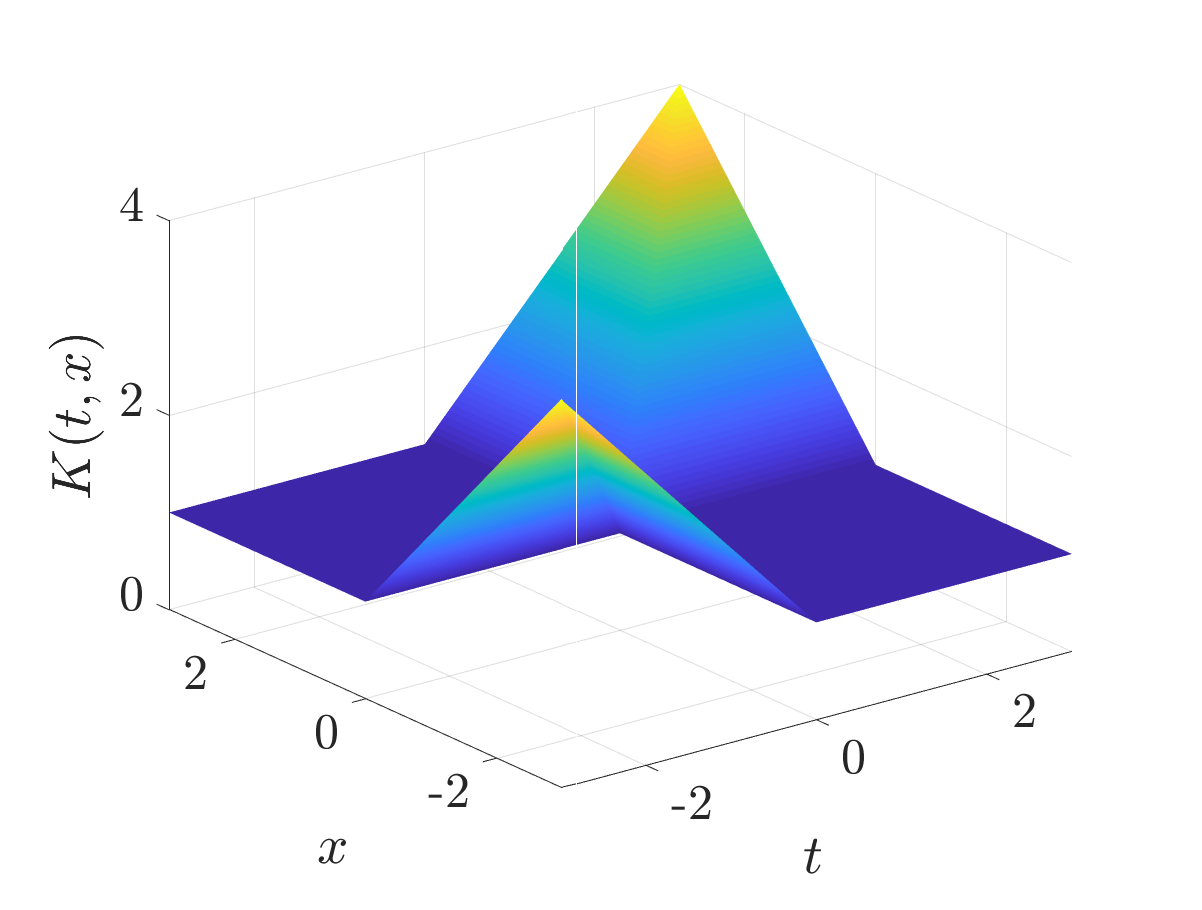
\includegraphics[height = 4cm]{code/Kernel3DPict.eps}
    \caption{The kernel defined in \eqref{eq:OrigKernel} for $d=1$.}
    \label{fig:kernelpict}
\end{figure}

The discrepancy for the uniform distribution on the unit cube defined in terms of the above kernel is commonly called the $L^2$ discrepancy and is expressed as
\begin{align} 
\nonumber
    D^2(\Udes,F_\unif,K)
    & = \int_{(0,1)^d \times (0,1)^d} K(\vt,\vx) \, \dif \vt \dif \vx - \frac 2N \sum_{i=1}^N \int_{(0,1)^d} K(\vt,\vu_i) \, \dif \vt\\
    \nonumber
    & \qquad \qquad  + \frac{1}{N^2} \sum_{i,k=1}^N K(\vu_i,\vu_k) \\
    \nonumber
    & = \left( \frac 43 \right)^d 
     - \frac 2N \sum_{i=1}^N \prod_{j=1}^d \left[1 + u_{ij} - \frac{u_{ij}^2}{2} \right] \\
     & \qquad \qquad + \frac 1{N^2} \sum_{i,k=1}^N \prod_{j=1}^d \left[1+ \min(u_{ij},u_{ik})\right]
\end{align}



%%%%%%%%%%%%%%%%%%%%%%%%%%%%%%%%%%%%%%%%%%%%%%%%%%%%%%%%%%%%%%%%%%%%%%%
\subsection{Definition in Terms of a Deterministic Cubature Error Bound}
\label{sec:DetermBound}
%%%%%%%%%%%%%%%%%%%%%%%%%%%%%%%%%%%%%%%%%%%%%%%%%%%%%%%%%%%%%%%%%%%%%%%

Now let $(\ch, \ip[\ch]{\cdot}{\cdot})$ be a reproducing kernel Hilbert space (RKHS) of functions \cite{Aro50}, $f: \Omega \rightarrow \mathbb{R}$, which appear as the integrand in \eqref{eq:integration}. By definition, the reproducing kernel, $K$, is the unique function defined on $\Omega \times \Omega$ with the properties that $K(\cdot, \vx)\in \ch$ for any $\vx \in \Omega$ and $f(\vx)=\ip[\ch]{K(\cdot,\vx)}{f}$.  This second property, implies that $K$ reproduces function values via the inner product. It can be verified that $K$ is symmetric in its arguments and positive definite as in \eqref{eq:sympd}.

The integral $\mu = \int_{\Omega} f(\vx) \, \varrho(\vx) \, \dif \vx$, which was identified as $\Ex[f(\vX)]$ in \eqref{eq:integration}, can be approximated by a sample mean, 
\begin{equation}\label{eq:cubature}
\hat{\mu}=\frac{1}{N}\sum_{i=1}^N f(\vx_i).
\end{equation}
The quality of this approximation to the integral, or cubature, depends in part on how well the empirical distribution of the design, $\Xdes = \{\vx_i\}_{i=1}^N$, matches the target distribution $F$ associated with the density function $\varrho$. 

Define the cubature error as  
\begin{align}
\nonumber 
\err(f,\Xdes) & = \mu - \hat{\mu} = \int_{\Omega} f(\vx)\, \varrho(\vx) \dif \vx -\frac{1}{N}\sum_{i=1}^N f(\vx_i) \\
& =\int_\Omega f(\vx) \, \dif[F(\vx)-F_{\Xdes}(\vx)]. \label{eq:err}
\end{align}
Under modest assumptions on the reproducing kernel,  $\err(\cdot, \Xdes)$ is a bounded, linear functional, so. 
by the Riesz representation theorem, there exists a unique representer, $\xi \in \ch$, such that 
\[
\err(f, \Xdes)=\ip[\ch]{f}{\xi}, \quad \forall f\in \ch.
\]
The reproducing kernel allows us to write down an explicit formula for that representer, namely, $\xi(\vx)=\ip[\ch]{K(\cdot,\vx)}{\xi}=\err(K(\cdot,\vx),\Xdes)$.
By the Cauchy-Schwarz inequality, there is a tight bound on the squared cubature error, namely
\begin{equation}\label{eq:wcErrA}
\abs{\err(f,\Xdes)}^2=\ip[\ch]{f}{\xi}^2\leq \norm[\ch]{f}^2 \norm[\ch]{\xi}^2.
\end{equation}
The first term on the right describes the contribution to the cubature error made by the nature of the integrand, while the second term describes the contribution made by the quality of the cubature rule.

The square norm of the representer of the error functional is 
\begin{align*}
\norm[\ch]{\xi}^2& =\ip[\ch]{\xi}{\xi}=\err(\xi,\Xdes) \quad \text{since $\err(\cdot,\Xdes)$ represents the error functional}\\
& = \err(\err(K(\cdot,\cdot \cdot),\Xdes),\Xdes) \quad \text{since } \xi(\vx)=\err(K(\cdot,\vx),\Xdes)\\
& =\int_{\Omega\times \Omega} K(\vt,\vx)\dif[F(\vx)-F_{\Xdes}(\vx)] \, \dif[F(\vt)-F_{\Xdes}(\vt)].
\end{align*}
We can equate this formula for $\norm[\ch]{\xi}^2$ with the formula for $D^2(\Xdes,F,K)$ in  \eqref{eq:discDef}.  Thus, the tight, worst-case cubature error  bound in \eqref{eq:wcErrA} can be written as
\begin{equation}\label{eq:wcErrB}
\abs{\err(f,\Xdes)} \le \norm[\ch]{f} D(\Xdes,F,K).
\end{equation}
This implies our second interpretation of the discrepancy in Table \ref{tab:ThreeInterpTable}.

We now identify the RKHS for the kernel $K$ defined in \eqref{eq:OrigKernel} Let $(\va,\vb)$ be some $d$ dimensional box containing the origin in the interior or on the boundary. For any $\fraku \subseteq \{1, \ldots, d\}$, define $\partial^\fraku f(\vx_\fraku) : = \partial^{|\fraku|}f(\vx_\fraku,\vzero)/\partial \vx_\fraku$, the mixed first-order partial derivative of $f$ with respect to the $x_j$ for $j\in \fraku$, while setting $x_j=0$ for all $j \notin \fraku$. Here, $\vx_{\fraku} = (x_j)_{j \in \fraku}$, and $|\fraku|$ denotes the cardinality of $\fraku$.  By convention, $\partial^{\emptyset}f := f(\vzero)$.  The inner product for the reproducing kernel $K$ defined in  \eqref{eq:OrigKernel} is defined as 
\begin{align}\label{eq:inner}
\langle f,g \rangle_{\ch} &:= \sum_{\fraku\subseteq \{1,...,d\}}\int_{(\va,\vb)}\partial^{\fraku}f(\vx_\fraku)\partial^{\fraku}g(\vx_\fraku) \, \dif \vx_\fraku \\
\nonumber
& = f(\vzero)g(\vzero)  + \int_{a_1}^{b_1} \partial^{\{1\}}f(x_1)\partial^{\{1\}}g(x_1) \, \dif x_1 \\
\nonumber 
& \qquad + \int_{a_2}^{b_2} \partial^{\{2\}}f(x_2)\partial^{\{2\}}g(x_2) \, \dif x_2 + \cdots \\
\nonumber 
& \qquad + \int_{a_2}^{b_2} \int_{a_1}^{b_1} \partial^{\{1,2\}}f(x_1,x_2)\partial^{\{1,2\}}g(x_1,x_2) \, \dif x_1 \dif x_2+ \cdots \\
\nonumber 
& \qquad + \int_{(\va,\vb)} \partial^{\{1,\ldots, d\}}f(\vx)\partial^{\{1, \ldots, d\}}g(\vx) \, \dif \vx. 
\end{align}

To establish that the inner product defined above corresponds to the reproducing kernel  $K$ defined in \eqref{eq:OrigKernel}, we note that
\begin{align*}
\partial^{\fraku} K((\vx_u,{\bf 0}),\vt) & =\prod_{j \in \fraku}\frac 12 \left[\sign(x_j) - \sign(x_j - t_j) \right] \\
& =
\prod\limits_{j \in \fraku}\sign(t_j) \bbone_{(\min(0,t_j),\max(0,t_j))}(x_j).
\end{align*}
Thus, $K(\cdot,\vt)$ possesses sufficient regularity to have finite $\ch$-norm.  Furthermore, $K$ exhibits the reproducing property for the above inner product because
\begin{align*}
\MoveEqLeft{\langle K(\cdot,\vt),f \rangle}_{\ch} \\
&= \sum_{\fraku\subseteq \{1,...,d\}}\int_{(\va,\vb)} \partial^{\fraku}K((\vx_u,{\bf 0}),\vt)\partial^{\fraku}f(\vx_u,{\bf 0})  \, \dif \vx_u \\
&= \sum_{\fraku\subseteq \{1,...,d\}}\int_{(\va,\vb)}  \prod\limits_{j \in \fraku}\sign(t_j) \bbone_{(\min(0,t_j),\max(0,t_j))}(x_j) \partial^{\fraku}f(\vx_u,{\bf 0})  \, \dif \vx_u \\
& =     \sum_{\fraku\subseteq \{1,...,d\}}\sum_{\frakv\subseteq \fraku}(-1)^{|\fraku|-|\frakv|}f(\vt_\frakv,{\bf 0})= f(\vt).
\end{align*}


%%%%%%%%%%%%%%%%%%%%%%%%%%%%%%%%%%%%%%%%%%%%%%%%%%%%%%%%%%%%%%%%%%%%%%%
\subsection{Definition in Terms of the Root Mean Squared Cubature Error}
\label{sec:RandomBound}
%%%%%%%%%%%%%%%%%%%%%%%%%%%%%%%%%%%%%%%%%%%%%%%%%%%%%%%%%%%%%%%%%%%%%%%

Assume $\Omega$ is a measurable subset in $\mathbb{R}^d$ and $F$ is the target probability distribution defined on $\Omega$ as defined earlier. 
Now, let $f: \Omega \rightarrow \mathbb{R}$ be a stochastic process with a constant pointwise mean, i.e., 
\[
\Ex_{f\in \mathcal{A}}[f(\vx)]=m, \qquad \forall \vx\in \Omega,
\]
where $\mathcal{A}$ is the sample space for this stochastic process. 
Now we interpret $K$ as the \emph{covariance kernel} for the stocastic process:
\[
K(\vt,\vx):=\Ex_{f\in \mathcal{A}}\left( [f(\vt)-m][f(\vx)-m]\right)=\cov(f(\vt),f(\vx)),\qquad \forall \vt, \vx\in \Omega. 
\]
It is straightforward to see that the kernel function is symmetric and positive definite. 

Define the error functional $\err(\cdot,\Xdes)$ in the same way as in \eqref{eq:err}.  Now, the mean squared error is 
\begin{align*}
&\Ex_{f\in\mathcal{A}}[(\err(f,\Xdes)]^2= \Ex_{f\in\mathcal{A}} \left\{\int_{\Omega}f(\vx)\dif F(\vx)-\frac{1}{N}\sum_{i=1}^N f(\vx_i) \right\}^2\\
=&\Ex_{f\in\mathcal{A}}\left\{\int_{\Omega}(f(\vx)-m)\dif F(\vx)-\frac{1}{N}\sum_{i=1}^N (f(\vx_i)-m) \right\}^2\\
=&\int_{\Omega^2}\Ex_{f\in \mathcal{A}}[ (f(\vt)-m)(f(\vx)-m)] \, \dif F(\vt)\dif F(\vx)\\
&-\frac{2}{N}\sum_{i=1}^N \int_{\Omega} \Ex_{f\in\mathcal{A}}[(f(\vx)-m)(f(\vx_i)-m)]\,\dif F(\vx)\\
&+\frac{1}{N^2}\sum_{i,k=1}^N\Ex_{f\in\mathcal{A}}[(f(\vx_i)-m)(f(\vx_k)-m)]\\
=&\int_{\Omega^2}K(\vt,\vx) \, \dif F(\vt)\dif F(\vx)-\frac{2}{N}\sum_{i=1}^N \int_{\Omega} K(\vx, \vx_i)\dif F(\vx)+\frac{1}{N^2} \sum_{i,k=1}^N K(\vx_i,\vx_k). 
\end{align*}
Therefore, we can equate the discrepancy $D(\Xdes, F, K)$ defined in \eqref{eq:discDef} as the root mean squared error:
\[
D(\Xdes, F, K) =\sqrt{\Ex_{f\in\mathcal{A}}[(\err(f,\Xdes)]^2}=\sqrt{\Ex\abs{\int_{\Omega}f(\vx)\varrho(\vx)\dif \vx-\frac{1}{N}\sum_{i=1}^N f(\vx_i)}^2}.
\]

%%%%%%%%%%%%%%%%%%%%%%%%%%%%%%%%%%%%%%%%%%%%%%%%%%%%%%%%%%%%%%%%%%%%%%%
\section{When Transformed Low Discrepancy Points Also Have Low Discrepancy}
%%%%%%%%%%%%%%%%%%%%%%%%%%%%%%%%%%%%%%%%%%%%%%%%%%%%%%%%%%%%%%%%%%%%%%%
Having motivated the definition of discrepancy in \eqref{eq:discDef} from three perspectives, we now turn our attention to the question posed in \eqref{BigQ}, namely, does a transformation of low discrepancy points with respect to the uniform distribution yield low discrepancy points with respect to the new target distribution. In this section, we show a positive result, yet recognize some qualifications.

Consider some symmetric, positive definite kernel, $K_\unif : (0,1)^d \times (0,1)^d \to \reals$, some uniform design $\Udes$, some other domain, $\Omega$, some other target distribution, $F$, and some transformation $\vPsi:(0,1)^d \to \Omega$ as defined in \eqref{eq:transPts}. Then the squared discrepancy of the uniform design can be expressed according to \eqref{eq:discDef} as follows:
\begin{align} 
\nonumber
    \MoveEqLeft{D^2(\Udes,F_{\unif},K_\unif)} \\
    \nonumber
    & = \int_{(0,1)^d \times (0,1)^d} K_\unif(\vu,\vv) \,  \dif \vu \dif \vv - \frac 2N \sum_{i=1}^N \int_{\Omega} K_\unif(\vu,\vu_i) \, \dif \vu\\
    \nonumber
    & \qquad \qquad  + \frac{1}{N^2} \sum_{i,k=1}^N K_\unif(\vu_i,\vu_k) \\
    \nonumber
    & = \int_{\Omega \times \Omega} K_\unif(\vPsi^{-1}(\vt),\vPsi^{-1}(\vx)) \, \abs{\frac{\partial \vPsi^{-1}(\vt)}{\partial \vt}} \abs{\frac{\partial \vPsi^{-1}(\vx)}{\partial \vx}} \,\dif \vt \dif \vx \\
    \nonumber 
    & \qquad \qquad  - \frac 2N \sum_{i=1}^N \int_{\Omega} K_\unif(\vPsi^{-1}(\vt),\vPsi^{-1}(\vx_i)) \, \abs{\frac{\partial \vPsi^{-1}(\vt)}{\partial \vt}} \, \dif \vt\\
    \nonumber
    & \qquad \qquad  + \frac{1}{N^2} \sum_{i,k=1}^N K_\unif(\vPsi^{-1}(\vx_i),\vPsi^{-1}(\vx_k)) \\
    & = D^2(\Xdes,F,K)
\end{align}
where the kernel $K$ is defined as
\begin{subequations} \label{eq:BigQYes}
\begin{equation} \label{eq:BigQYesa}
    K(\vt,\vx) = K_{\unif}(\vPsi^{-1}(\vt),\vPsi^{-1}(\vx))
\end{equation}
\emph{and provided that} the density, $\varrho$, corresponding to the target distribution, $F$, satisfies
\begin{equation} \label{eq:BigQYesb}
    \varrho(\vx) = \abs{\frac{\partial \vPsi^{-1}(\vx)}{\partial \vx}}
\end{equation}
\end{subequations}
The above argument is summarized in the following theorem.

\begin{theorem}
Suppose that the design $\Xdes$ is constructed by transforming the design $\Udes$ according to the transformation \eqref{eq:transPts}.  Also suppose that conditions \eqref{eq:BigQYes} are satisfied.  Then $\Xdes$ has the same discrepancy with respect to the target distribution, $F$, defined by the kernel $K$ as does the original design $\Udes$ with respect to the uniform distribution and defined by the kernel $K_\unif$.  That is,
\begin{equation}
     D(\Xdes,F,K) = D(\Udes,F_{\unif},K_\unif)
\end{equation}
As a consequence, under conditions \eqref{eq:BigQYes}, question \eqref{BigQ} has a positive answer.
\end{theorem}

Condition \eqref{eq:BigQYesb} may be easy to satisfy.  For example, it is automatically satisfied by the inverse cumulative distribution transform \eqref{eq:inverse}.  Condition \eqref{eq:BigQYesa} is simply a matter of definition of the kernel, $K$, but it is definition with consequences.  From the perspective of Section \ref{sec:HilbertMeasures}, changing the kernel means changing the definition of the distance between two Dirac measures.  From the perspective of Section \ref{sec:DetermBound}, changing the kernel means changing the definition of the Hilbert space of integrands, $f$, in \eqref{eq:integration}.   From the perspective of Section \ref{sec:RandomBound}, changing the kernel means changing the definition of the covariance kernel for the integrands, $f$, in \eqref{eq:integration}.

To illustrate this point, consider a cousin of the kernel in \eqref{eq:OrigKernel}, which places the reference point at $\boldsymbol{0.5} = (0.5, \ldots, 0.5)$, the center of the unit cube $(0,1)^d$:
\begin{align}
\label{eq:L2kernel}
    K_{\unif}(\vu,\vv) &= \prod_{j=1}^d\left[1+\frac{1}{2}\left(\left|u_j-1/2\right|+ \left|v_j- 1/2 \right|-\left |u_j-v_j \right| \right) \right] \\
    \nonumber
    & = K(\vu - \boldsymbol{0.5}, \vv - \boldsymbol{0.5}) \qquad \text{for $K$ defined in \eqref{eq:OrigKernel}}. 
\end{align}
This kernel defines the centered $L^2$-discrepancy \cite{Hic97a}.
Consider the standard multivariate normal distribution, $F_\normal$, and choose the inverse normal distribution,
\begin{equation} \label{eq:invNormTrans}
    \vPsi(\vu) = (\Phi^{-1}(u_1), \ldots, \Phi^{-1}(u_d)),
\end{equation}
where $\Phi$ denotes the standard normal distribution function.  Then condition \eqref{eq:BigQYesb} is automatically satisfied, and condition \eqref{eq:BigQYesa} is  satisfied by defining
\begin{align}
\nonumber
     K(\vt,\vx) &= K_{\unif}(\vPsi^{-1}(\vt),\vPsi^{-1}(\vx)) \\
     \nonumber
      &= \prod_{j=1}^d\left[1+\frac{1}{2}\left(\left|\Phi(t_j)-1/2\right|+ \left|\Phi(x_j)- 1/2 \right| \right . \right . \\
      & \qquad \qquad \left.  \left . -\left|\Phi(t_j)-\Phi(x_j)\right|\right)\right].
\end{align}
In one dimension, the distance between two Dirac measures defined using the kernel $K_\unif$ above is $\norm{\delta_{x} - \delta_{t}} = \sqrt{|x-t|}$, whereas the distance defined using the kernel $K$ above is $\norm{\delta_{x} - \delta_{t}} = \sqrt{|\Phi(x)-\Phi(t)|}$. Under kernel $K$, the distance between two Dirac measures can never be greater than one.  Such an assumption may be unpalatable.

%%%%%%%%%%%%%%%%%%%%%%%%%%%%%%%%%%%%%%%%%%%%%%%%%%%%%%%%%%%%%%%%%%%%%%%
\section{Do Transformed Low Discrepancy Points Have Low Discrepancy More Generally}
%%%%%%%%%%%%%%%%%%%%%%%%%%%%%%%%%%%%%%%%%%%%%%%%%%%%%%%%%%%%%%%%%%%%%%%

From the discussion above indicates that condition \eqref{eq:BigQYesa} can be too restrictive.  We would like to compare the discrepancies of designs under kernels that do not satisfy that restriction.  In particular, we consider the centered $L^2$-discrepancy for uniform designs on $(0,1)^d$ defined by the kernel in \eqref{eq:L2kernel}:
\begin{align*}
\MoveEqLeft{D^2(\Udes, F_\unif, K_\unif)} \\
& = \left(\frac{13}{12}\right)^d - \frac{2}{N}\sum_{i=1}^N \prod_{j=1}^d \left[1+\frac{1}{2}\left(|u_{ij}-1/2|-|u_{ij}-1/2|^2\right) \right]\\
& \qquad + \frac{1}{N^2}\sum_{i,k=1}^N\prod_{j=1}^d\left[1+\frac{1}{2}\left(|u_{ij}-1/2|+|u_{kj}-1/2|-|u_{ij}-u_{kj}| \right) \right],  
\end{align*}
where again, $F_\unif$ denotes the uniform distribution on $(0,1)^d$, and $\Udes$ denotes a design on $(0,1)^d$

Changing perspectives slightly, if $F_\unif'$ denotes the uniform distribution on the cube of volume one centered at the origin, $(-0.5,0.5)^d$, and the design $\Udes'$ is constructed by  subtracting $\boldsymbol{0.5}$ from each point in the design $\Udes$:
\begin{equation} \label{eq:Updef}
    \Udes' = \{\vu -\boldsymbol{0.5} : \vu \in \Udes \},
\end{equation}
then 
\begin{equation} \label{eq:desEquiv}
     D(\Udes',F'_\unif,K) = D(\Udes, F_\unif, K_\unif),
\end{equation}
where $K$ is the kernel defined above in \eqref{eq:OrigKernel}.  Recall that the origin is a special point in the definition of the inner product corresponding to this $K$ as a reproducing kernel in \eqref{eq:inner}.

Therefore, this $K$ from \eqref{eq:OrigKernel} is an appropriate kernel to use to define the the discrepancy for designs defined with respect to the standard normal distribution, which is also centered at the origin.  Such a discrepancy is 
\begin{align}\label{eq:DisNormald>1}
\nonumber
\MoveEqLeft{D^2(\Xdes, F_\normal, K) = \left(1+\sqrt{\frac{2}{\pi}}\right)^d}\\
\nonumber
  & - \frac{2}{N}\sum_{i=1}^N \prod\limits_{j=1}^d\left[ 1+\frac{1}{\sqrt{2\pi}}+\frac{1}{2}|x_{ij}|-x_{ij}\left(\Phi(x_{ij})-\frac 12 \right)-\phi(x_{ij})\right]\\
  &+\frac{1}{N^2}\sum_{i,k=1}^N \prod_{j=1}^d \left[1+\frac{1}{2}\left(|x_{ij}|+|x_{kj}|-|x_{ij}-x_{kj}|\right)\right]. 
\end{align}
Here, $\phi$ is the standard normal probability density function. 
The derivation of \eqref{eq:DisNormald>1} is given in the Appendix. 

%\section{Inconsistency in Discrepancy}\label{sec:inconsistency}
Now we numerically compare the discrepancy of a uniform design, $\Udes'$ given by \eqref{eq:Updef} and the discrepancy of a design constructed by the inverse normal transformation, i.e.,  $\Xdes = \vPsi(\Udes)$ for $\vPsi$ in \eqref{eq:invNormTrans}, where the $\Udes$ leading to both is identical.  We do not expect the magnitudes of the discrepancies to be the same, but we ask
\begin{multline} \tag{Q'} \label{eq:BigQPrime}
    \text{does } D(\Udes'_1,F'_\unif, K)\leq D(\Udes_2',F_\unif', K) \\
    \text{imply }
     D(\vPsi(\Udes_1),F_\normal, K)\leq D(\vPsi(\Udes_2),F_\normal, K)?
\end{multline}
Again, $K$ is given by \eqref{eq:OrigKernel}.  So we are actually comparing discrepancies defined by the same kernels, but \emph{not kernels that satisfy \eqref{eq:BigQYesa}}.

Let $d=5$ and $N=50$. 
We generate $B=20$ independent and identically distributed (IID) uniform designs, $\Udes$ with $N=50$ points on $(0,1)^5$ and then use the inverse distribution transformation to obtain IID random $N({\bf 0}, {\mathsf I}_5)$ designs, $\Xdes = \vPsi(\Udes)$. 
Figure \ref{fig:UniVsNormDisc} plots the discrepancies for normal designs, $D(\vPsi(\Udes),F_\normal, K)$,  against the discrepancies for the uniform designs, $D(\Udes,F_\unif,K_\unif) = D(\Udes',F_\unif',K)$ for each of the $B=20$ designs. 
Question \eqref{eq:BigQPrime} has a positive answer if and only if the lines passing through any two points on this plot should all have non-negative slope.  However, that is not the case.  Thus \eqref{eq:BigQPrime} is false.

\begin{figure}[ht]
\begin{center}
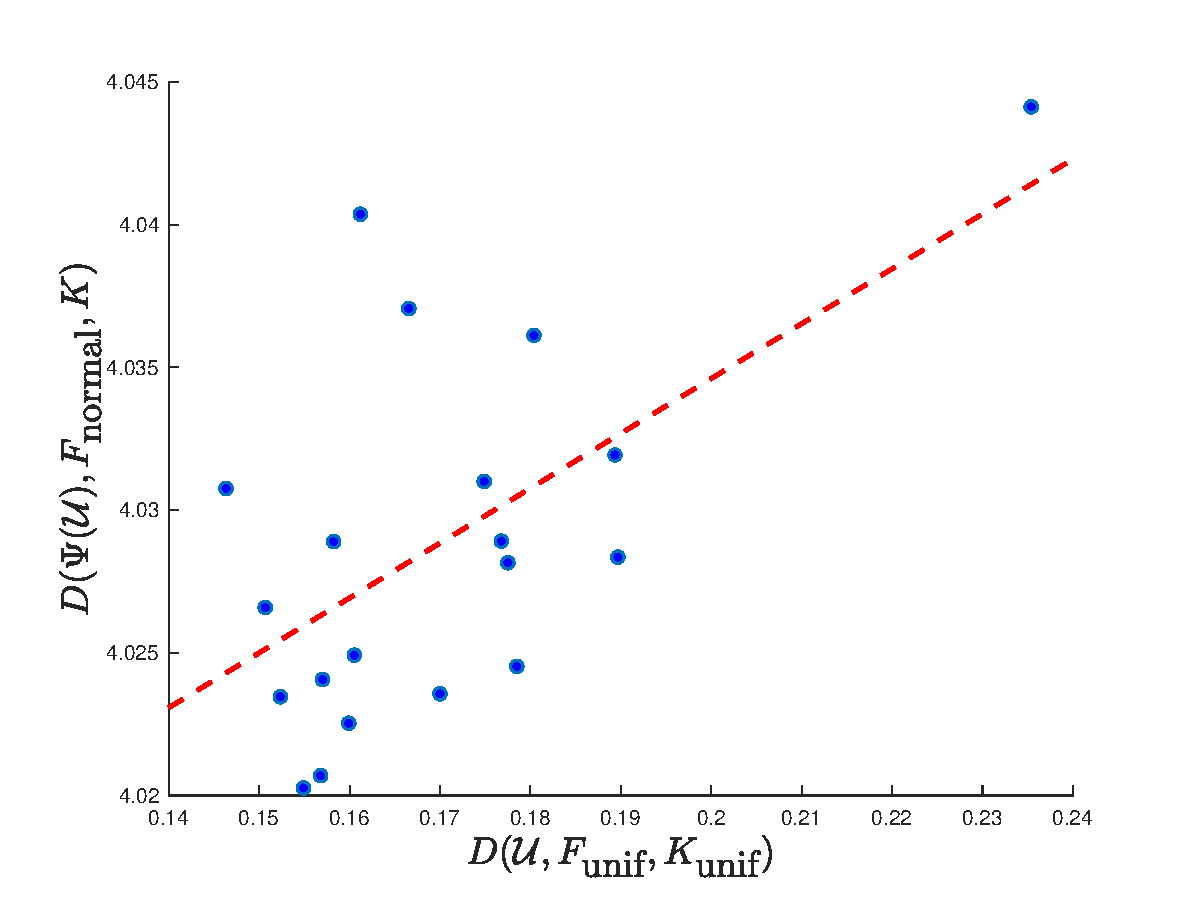
\includegraphics[width=8cm]{code/d5n50.eps}
\caption{Uniform Discrepancy Vs. Normal Discrepancy. \label{fig:UniVsNormDisc}}
\end{center}
\end{figure}

We further investigate the relationship between the discrepancy of a uniform design and the  discrepancy of the same design after inverse normal transformation.
Varying the dimension $d$ from $1$ to $10$, we calculate the sample correlation between $D(\vPsi(\Udes),F_\normal, K)$ and $D(\Udes,F_\unif,K_\unif) = D(\Udes',F_\unif',K)$ for $B=500$ IID designs of size $N=50$.  Figure \ref{fig:DiscVsd} displays the correlation as a function of $d$. Although the correlation is positive, it degrades with increasing $d$.

\begin{figure}[ht]
\begin{center}
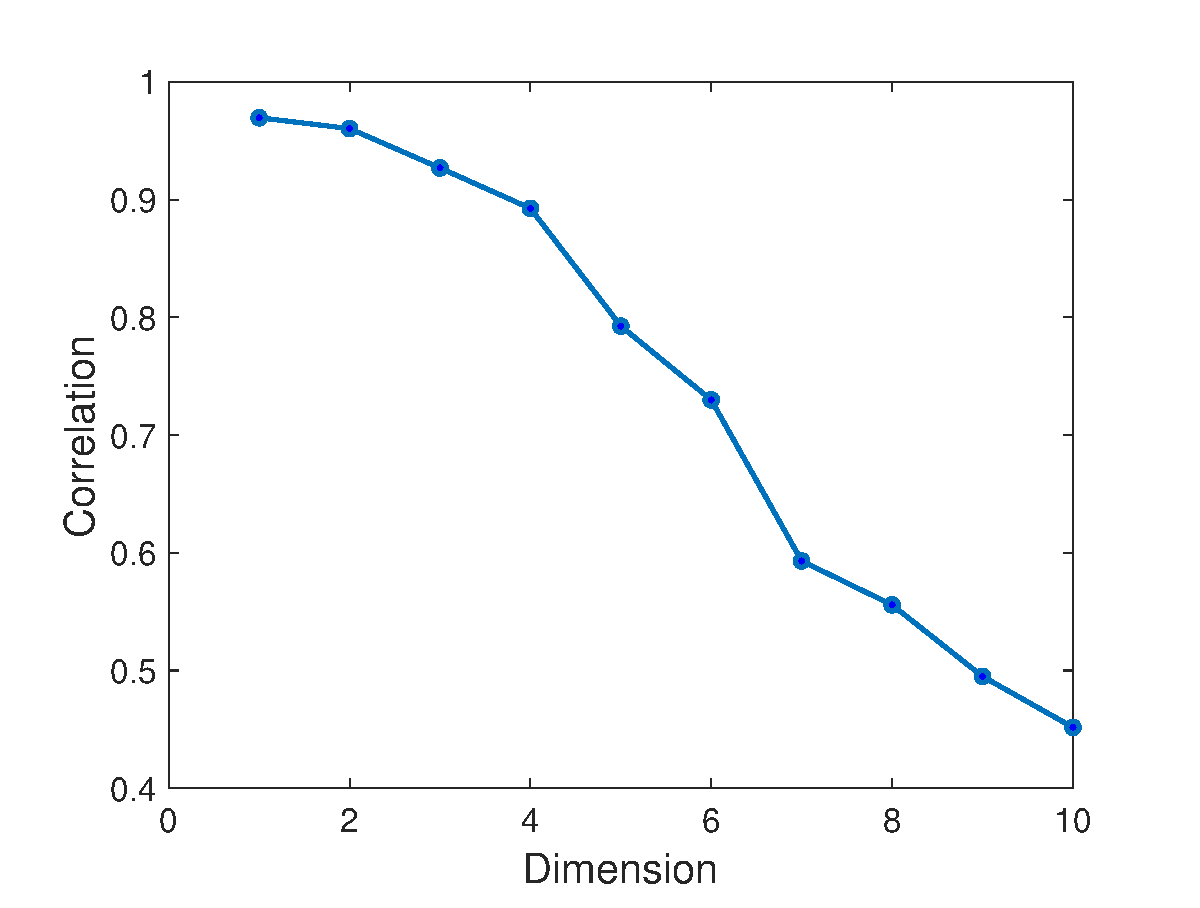
\includegraphics[width=8cm]{code/dimVsdisc.eps}
\caption{Correlation between Uniform Discrepancy and Normal Discrepancy with Different Variable Dimensions. \label{fig:DiscVsd}}
\end{center}
\end{figure}

\FJH{Fred does not understand this example.}
A simple example of integral approximation below shows that a naively inverse transformed sequence $\Udes$ could result in very misleading estimate even if $D(\Udes,F_\unif, K)$ is small.

\emph{Example}: Consider estimating the integral
\begin{align}\label{eq:badexample}
\int_{\mathbb{R}^d} \frac{x_1+\cdots+x_d}{1+10^{-8}(x_1^2+\cdots+x_d^2)}\dif \Phi(\vx) & = \Ex\left[\frac{\sum\limits_{i=1}^d x_i}{1+10^{-8}\|\vx\|_2^2}\right],\,\,\,\vx\sim N({\bf 0}, {\mathsf I}_d)
\end{align}
using Monte Carlo method, with $d=10$ and $N=2^{10}$ points. Analytically, the integral \eqref{eq:badexample} equals 0 since $\frac{x_1+\cdots+x_d}{1+10^{-8}(x_1^2+\cdots+x_d^2)}$ is an odd function in each dimension and the probability density function of standard normal is an even function. We start with two uniform random sequences. One is a Sobol sequence that has small uniform discrepancy, denoted as $\Udes_1$. Then we move the closest point to origin $0^d$ in $\Udes_1$ to $\left(10^{-15}\right)^d$, and denote the new sequence as $\Udes_2$. We compare the integral estimate with samples $\vPsi(\Udes_1)$ and $\vPsi(\Udes_2)$. Table \ref{tab:badexample} shows that the uniform discrepancies of $\Udes_1$ and $\Udes_2$ don't differ much, but the normal discrepancy of $\vPsi(\Udes_2)$ is far larger than that of $\vPsi(\Udes_1)$. In return, the estimate error corresponding to $\Udes_2$ is about 60 times larger than that corresponding to $\Udes_1$.

% Table generated by Excel2LaTeX from sheet 'Sheet1'
\begin{table}[htbp]
  \centering
  \caption{Comparison of Integral Estimate}
    \begin{tabular}{ccccc}
    \hline
   $\Udes$       & $D(\Udes,F_\unif, K)$     & $D(\vPsi(\Udes),F_\normal, K)$     & Estimate \\
    \hline
    $\Udes_1$     &   0.0285    &  18.57     & 0.0011 \\
    $\Udes_2$     &  0.0292      &  58.82     & -0.0660 \\
    \hline
    \end{tabular}%
  \label{tab:badexample}%
\end{table}%

\section{Improvement by the Coordinate-Exchange Method}\label{sec:CoordEx}

In this section, we propose an efficient algorithm that improves the design's quality in terms of the discrepancy for the target standard normal distribution. 
We start with a low-discrepancy uniform design, such as a Sobol sequence, and apply the inverse transformation to the design so that the transformed design approximates the target distribution, which is the standard normal distribution in this work. 
Following the optimal design approach, we consider the discrepancy of the normal design as the design criterion and apply a certain optimization algorithm to further improve the design, until the discrepancy reaches the minimum.

The optimization algorithm we choose is the coordinate-exchange algorithm, which was firstly introduced in \cite{meyer1995coordinate}, and then applied widely to construct various kinds of optimal design \cite{sambo2014coordinate,overstall2017bayesian,kang2018stochastic}. 
The coordinate-exchange algorithm is an iterative optimization method.
It finds the ``worst" coordinate $x_{ij}$ of the current design and replace it with a better coordinate that decreases the discrepancy. 
The most appealing advantage of the coordinate-exchange algorithm is that at each step one need only solve a univariate optimization problem.

First, we define the point deletion function, $\frakd_p$, as the change in square discrepancy resulting from removing the a point from the design:
\begin{equation}\label{eq:rowdeletion}
\frakd_p(i) = D^2(\Xdes)-\left(\frac{N-1}{N}\right)^2 D^2(\Xdes\backslash \{\vx_i\}).
\end{equation}
Here, the design $\Xdes\backslash \{\vx_i\}$ is the $N-1$ point design with the point $\{\vx_i\}$ removed. We suppress the choice of target distribution and kernel in the above discrepancy notation for simplicity. We then choose 
\begin{equation} \label{eq:rowchoice}
    i^*=\argmax_{i=1,\ldots,N} \frakd_p(i).
\end{equation}
The definition of $i^*$ means that removing $\vx_{i^*}$ from the design $\Xdes$ results in the smallest discrepancy among all possible deletions.  Thus, $\vx_{i^*}$ is helping the least, which makes it a prime candidate for modification.

Next, we define a coordinate deletion function, $\frakd_{c}$, as the change in the square discrepancy resulting from removing a coordinate in our calculation of the discrepancy:
\begin{equation}\label{eq:coorddeletion}
\frakd_c(k) = D^2(\Xdes)-D^2(\Xdes_{-k}).
\end{equation}
Here, the design $\Xdes_{-k}$ still has $N$ points but now only $d$ dimensions, the $k^{\text{th}}$ coordinate having been removed.  For this calculation to be feasible, we need the target distribution to independent marginals defined on the domain.  Also, the kernel to be of product form.  To simplify the notation, we assume a somewhat stronger condition, namely that each term in the product defining the kernel is the same for every coordinate:
\begin{equation}
    \label{eq:prodkernel}
    \Omega = \tOmega \times \cdots \times \tOmega, \qquad K(\vt,\vx) = \prod_{k=1}^d [1+ \tK(t_k,x_k)], \qquad \tK:\tOmega \times \tOmega \to \reals.
\end{equation}
where the term in the product is 
We then choose 
\begin{equation} \label{eq:rowchoice}
    k^*=\argmax_{k=1, \ldots, d} \frakd_c(k).
\end{equation}
For reasons analogous to those given above, the $k^{*\text{th}}$ coordinate seems the best candidate for change.

Let $\Xdes^*(x)$ denote the design that results from replacing $x_{i^*k^*}$ by $x$.  We now define $\Delta(x)$ as improvement in the squared discrepancy resulting from replacing $\Xdes$ by $\Xdes^*(x)$:
\begin{equation}\label{eq:deltafun}
\Delta(x) = D^2(\Xdes)-D^2(\Xdes^*(x)).
\end{equation}
If we can find an $x$ for which $\Delta(x)$ is positive, then we can reduce the discrepancy.  This is the rationale for the coordinate-exchange algorithm given in  Algorithm \ref{alg:coorex}. 

\begin{algorithm}[ht]
\caption{Coordinate Exchange Algorithm.\label{alg:coorex}}
\begin{algorithmic}[1]
\INPUT An initial design $\Xdes$ on the domain $\Omega$, a target distribution, $F$, and a kernel, $K$ of the form \eqref{eq:prodkernel}, a small value $TOL$ to measure convergence of the algorithm, and the maximum allowed number of iterations, $I_{\max}$.
\OUTPUT Low discrepancy design $\Xdes$. 
\State Compute the squared discrepancy $D^2_0$ for the initial design $\Xdes$ and set the iteration index $i=0$.
\For{$i=1,2,\ldots, I_{\max}$}
\State Compute the point deletion function $\frakd_p(1), \ldots, \frakd_p(N)$. Choose the $i^*$-th point which has the largest point deletion value, i.e. $i^* = \argmax_{i} \frakd_p(i)$. 
\State For the $i^*$-th point, Compute the coordinate deletion function $\frakd_c(1), \ldots, \frakd_c(d)$ and choose the $j^*$-th element which has the largest coordinate deletion value, i.e., $k^* = \argmax_{k} \frakd_c(k)$. 
\State Replace the coordinate $x_{i^*k^*}$ by $x^*$ which is the solution of the univariate optimization
\[
x^* = \argmax_{x \in \tOmega} \Delta(x).
\]
\If{$\Delta(x^*)/D^2_{i-1}>TOL$} 
\State {Replace $x_{i^*k^*}$ with $x^*$ in the design $\Xdes$, i.e., let  $\Xdes(x^*)$ replace the old $\Xdes$.}
\State Update the squared discrepancy $D^2_{i}=D^2_{i-1}-\Delta(x^*)$. 
\Else 
\State{Terminate the loop and return the design $\Xdes$.} 
\EndIf
\EndFor
\end{algorithmic}
\end{algorithm}

For kernels of product form, \eqref{eq:prodkernel}, and target distributions with independent and identical marginals, the formula for the squared discrepancy in \eqref{eq:discDef} becomes
\begin{align}
\nonumber
    D^2(\Xdes,\rho,K)  & = (1+c)^d  - \frac 2N \sum_{i=1}^N H(\vx_{i}) + \frac{1}{N^2}  \sum_{i,j=1}^N K(\vx_{i},\vx_{j}),
    \intertext{where}
    h(x) & = \int_{\tOmega} \tK(t,x)  \, \tvarrho(t) \, \dif t, \\
    c & = \int_{\tOmega \times \tOmega} \tK(t_k,x_k) \, \tvarrho(t) \tvarrho (x) \, \dif t\dif x = \int_{\tOmega} h(x) \, \tvarrho(x) \, \dif x, \\
    H(\vx) &= \prod_{k=1}^d [1+ h(x_{k})].
\end{align}
An evaluation of $h(x)$ and $\tK(t,x)$ each require $\Order(1)$ operations, while an evaluation of $H(\vx)$ and $K(\vt,\vx)$ each require $\Order(d)$ operations.  The computation of $D(\Xdes,\rho,K)$ requires $\Order(dN^2)$ operations because of the double sum.
For a standard multivariate normal target distribution and the kernel defined in \eqref{eq:OrigKernel}, we have
\begin{align*}
c &= \sqrt{\frac{2}{\pi}}, \\
h(x) &= \frac{1}{\sqrt{2\pi}}+\frac{1}{2}|x|-x[\Phi(x)-1/2]-\phi(x),\\
\tK(t,x) &= \frac{1}{2} (|t|+ |x|- |x-t|).
\end{align*}

The point deletion function defined in \eqref{eq:rowdeletion} then can be expressed as
\begin{align}
\nonumber
\frakd_p(i) 
&= \frac{(2N-1)(1+c)^d}{N^2} - \frac{2}{N}\biggl[ \frac{1}{N} \sum_{j=1}^N  H(\vx_{j}) + \left(1 - \frac 1N \right) H(\vx_{i})  \biggr] \\
\label{eq:rowdeletionA}
& \qquad \qquad + \frac{1}{N^2}\biggl[2 \sum_{j=1}^N K(\vx_{i},\vx_{j})- K(\vx_{i},\vx_{i})\biggr]. 
\end{align}
The computational cost for $\frakd_p(1), \ldots, \frakd_p(N)$ is then $\Order(dN^2)$, which is the same order as the cost of the discrepancy of a single design.

The coordinate deletion function defined in \eqref{eq:coorddeletion} can be be expressed as
\begin{multline}\label{eq:coldeletionA}
\frakd_c(k) = (c-1)c^{d-1} -\frac{2}{N}\sum_{i=1}^N \frac{h(x_{ik})H(\vx_i)}{1+h(x_{ik})}  \\
+\frac{1}{N^2}\sum_{i,j=1}^N \frac{\tK(x_{ik},x_{jk}) K(\vx_i,\vx_j)}{1+\tK(x_{ik},x_{jk})}  .
\end{multline}
The computational cost for $\frakd_c(1), \ldots, \frakd_p(d)$ is also $\Order(dN^2)$, which is the same order as the cost of the discrepancy of a single design.


Finally, the  function $\Delta$ defined in \eqref{eq:deltafun} is given by
\begin{align}\label{eq:deltafunction}
\nonumber
\Delta(x)
&= -\frac{2\left[  h(x_{i^*k^*})-h(x)    \right]H(\vx_{i^*})}{N[1 + h(x_{i^*k^*})]}   \\
\nonumber
& \qquad \qquad +\frac{1}{N^2}\left(2\sum_{\substack{i=1 \\ i \ne i^*}}^N  \frac{[\tK(x_{i^*k^*},x_{ik^*})-\tK(x,x_{ik^*})] K(\vx_{i^*},\vx_i)} {1 + \tK(x_{i^*k^*},x_{ik^*})} \right . \\
& \qquad \qquad \left . + \frac{[\tK(x_{i^*k^*},x_{i^*k^*})-\tK(x,x)] K(\vx_{i^*},\vx_{i^*})} {1 + \tK(x_{i^*k^*},x_{i^*k^*})} \right )
\end{align} 
If we drop the terms that are independent of $x$, then we can maximize the function
\begin{equation}\label{eq:deltapfunction}
\Delta'(x) = Ah(x)  - \frac{1}{N}\sum_{\substack{i=1 \\ i \ne i^*}}^N B_i \tK(x,x_{ik^*}) - C \tK(x,x)
\end{equation}
where
\begin{equation*}
A = \frac{2H(\vx_{i^*})}{1 + h(x_{i^*k^*})}, \quad
B_i  = \frac{2K(\vx_{i^*},\vx_i)} {1 + \tK(x_{i^*k^*},x_{ik^*})}, \quad
C  = \frac{K(\vx_{i^*},\vx_{i^*})} {N[1 + \tK(x_{i^*k^*},x_{i^*k^*})]}.
\end{equation*}
Note that $A, B_1, \ldots, B_N, C$ only need to be computed once for each iteration of the coordinate exchange algorithm.

\FJH{Fred got to here}


\section{Simulation}

To demonstrate the performance of the $d$-dim standard normal design proposed in Section \ref{sec:CoordEx}, we compare three algorithms: (1) RAND: inverse transformed uniform random sequence;  (2) SOBOL: inverse transformed Sobol sequence; (3) E-SOBOL: inversed transformed scrambled Sobol sequence with uni-dimensional projection at $\left\{\frac{2i-1}{2N}\right\}_{i=1}^{2N}$; (4) CE: improved E-SOBOL with proposed Algorithm 1. 
We have tried different combinations of dimension and sample size, and let the sample size become larger as the dimension becomes higher. 
Using each algorithm we generate 500 designs, and for each design, we compute the discrepancy \eqref{eq:DisNormald>1} and compare the distribution of discrepancies from different algorithms as shown in Figure \ref{fig:comparison}. 

Figure \ref{fig:SOBOLVsRAND} contains the boxplots of normal discrepancies corresponding to the four generators with $d=2$ and $N=32$. It shows that SOBOL, E-SOBOL and CE all outperform RAND by a great margin. To better present the comparison between the generators, in the follow figures, we exclude the boxplot from RAND.

\begin{figure}[ht]
\begin{center}
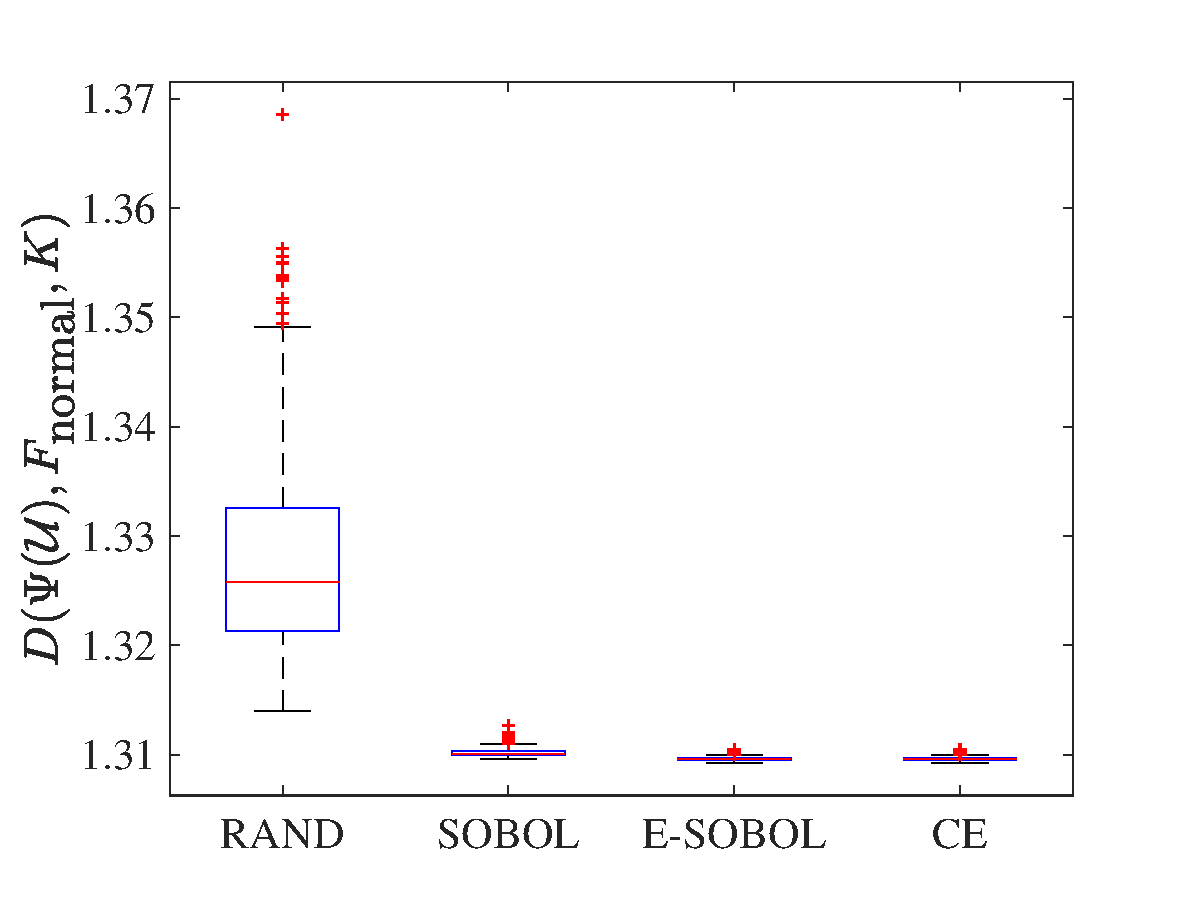
\includegraphics[width=8cm]{code/boxplotall_d2n32.eps}
\caption{Performance Comparison of Generators. \label{fig:SOBOLVsRAND}}
\end{center}
\end{figure}

We summarize the observations as follows. 
\begin{enumerate}
\item
Overall, E-SOBOL and CE outperform SOBOL. 
\item 
When the sample is relatively dense, i.e., $N/d$ ratio is large, E-SOBOL and CE have similar performance. They both outperform SOBOL by a great margin
\item
As the sample becomes more sparse, i.e., $N/d$ ratio is smaller, SOBOL and E-SOBOL have similar performance. The proposed CE becomes much superior to both of them.
\end{enumerate}
Therefore, E-SOBOL sequences are preferable when the sample size is large relative to the dimension, and we recommend using the proposed remedy approach to further improve E-SOBOL when the sample size is small or moderate. 

\begin{figure}[ht]\label{fig:comparison}
\centering
{\subfigure[$d=2,N=32$] {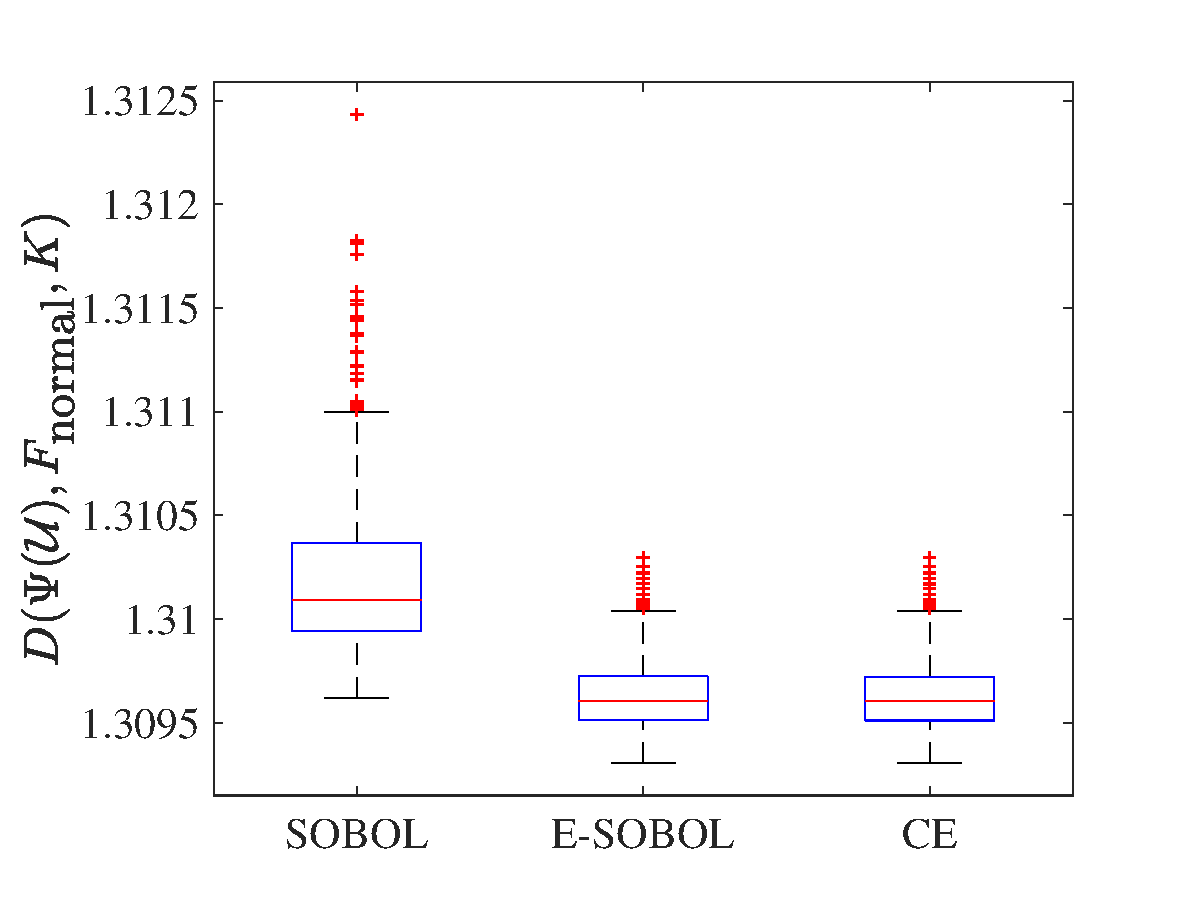
\includegraphics[width=5.5cm]{code/boxplot_d2n32.eps}}}
\quad
{\subfigure [$d=3, N=64$]
{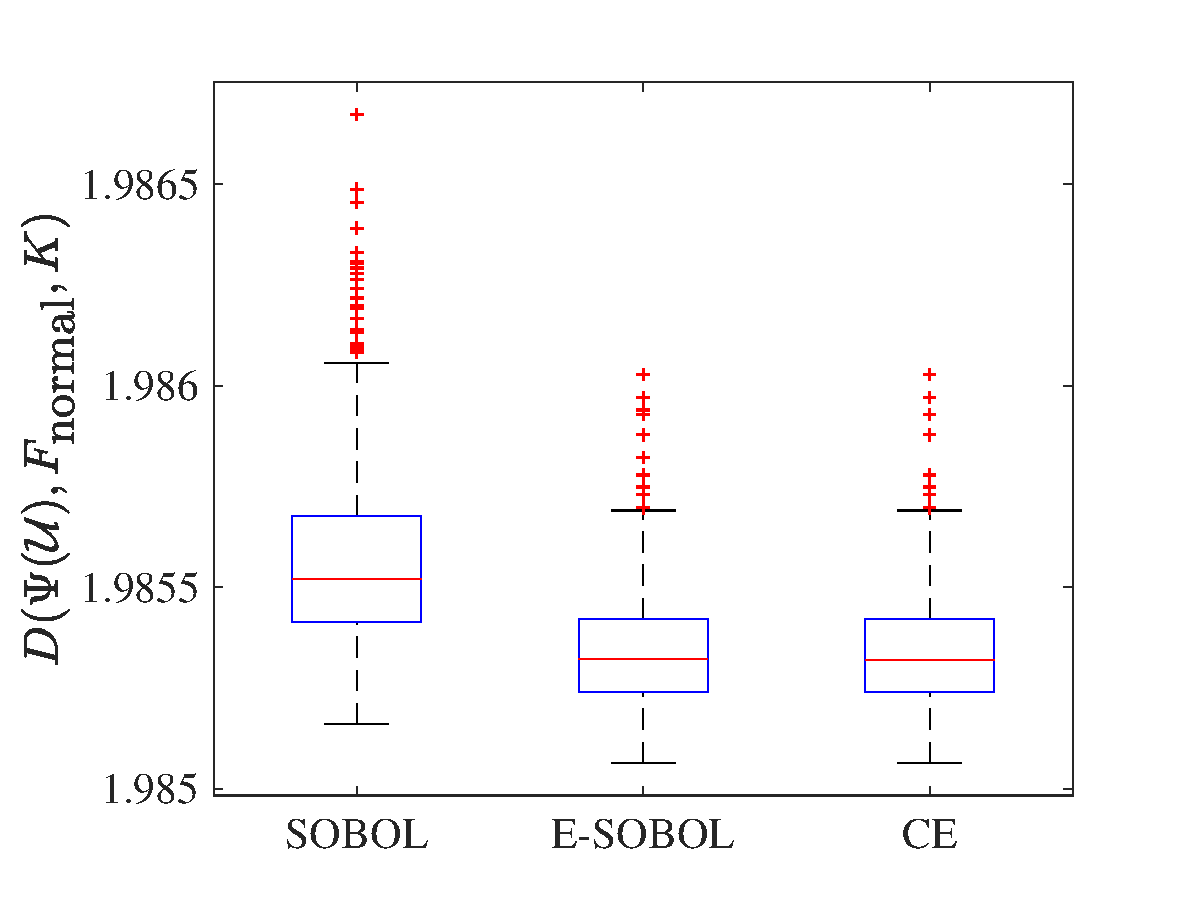
\includegraphics[width=5.5cm]{code/boxplot_d3n64.eps}}}
\quad
{\subfigure[$d=4, N=64$] {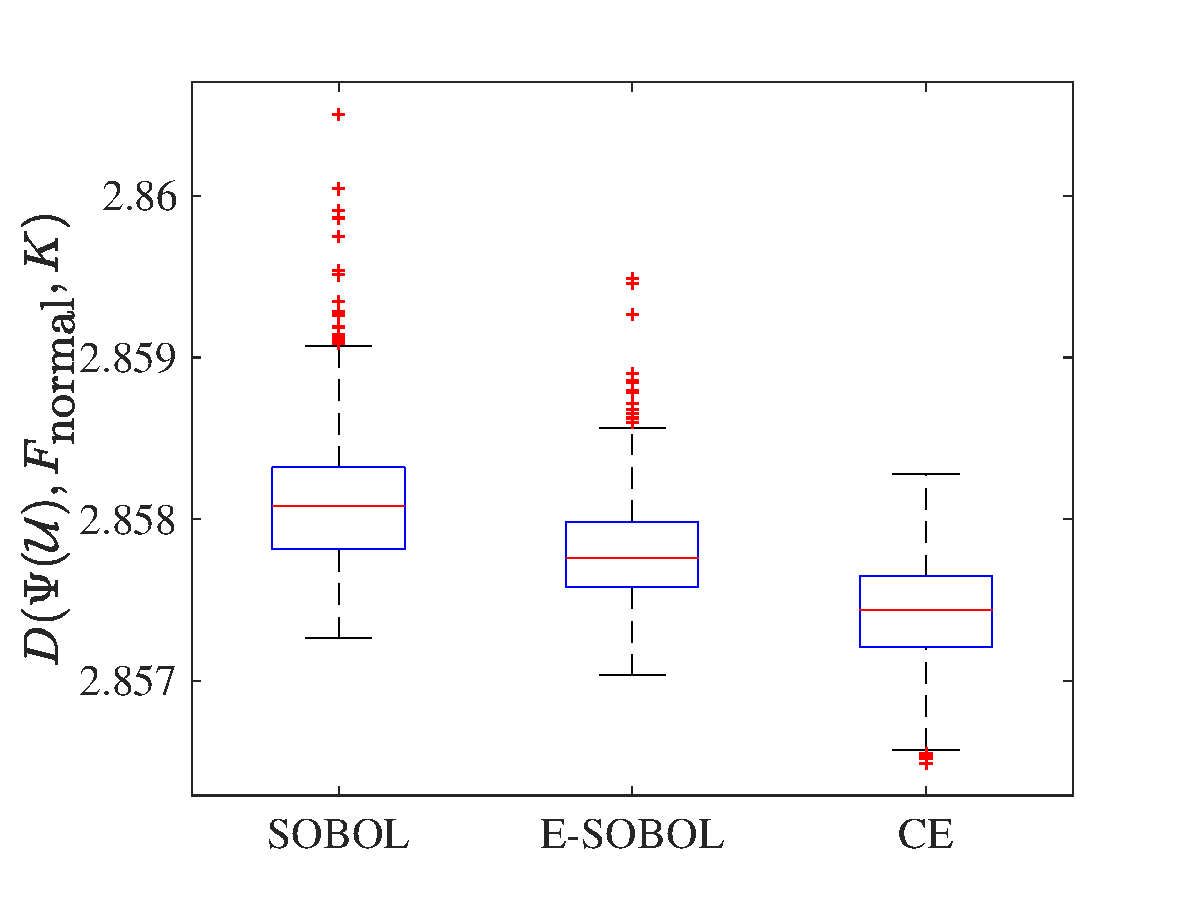
\includegraphics[width=5.5cm]{code/boxplot_d4n64.eps}}}
\quad
{\subfigure[$d=6, N=128$] {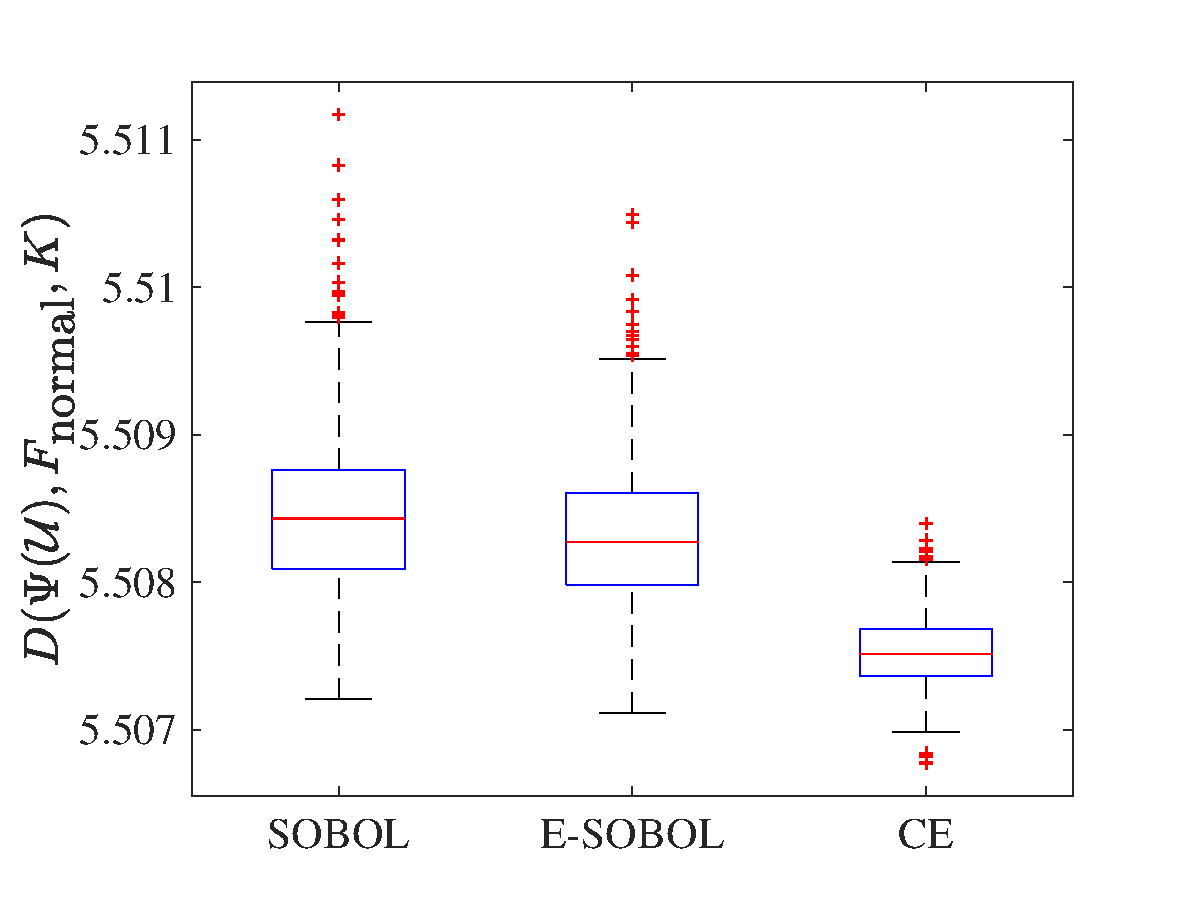
\includegraphics[width=5.5cm]{code/boxplot_d5n128.eps}}}
\quad
{\subfigure[$d=8, N=256$] {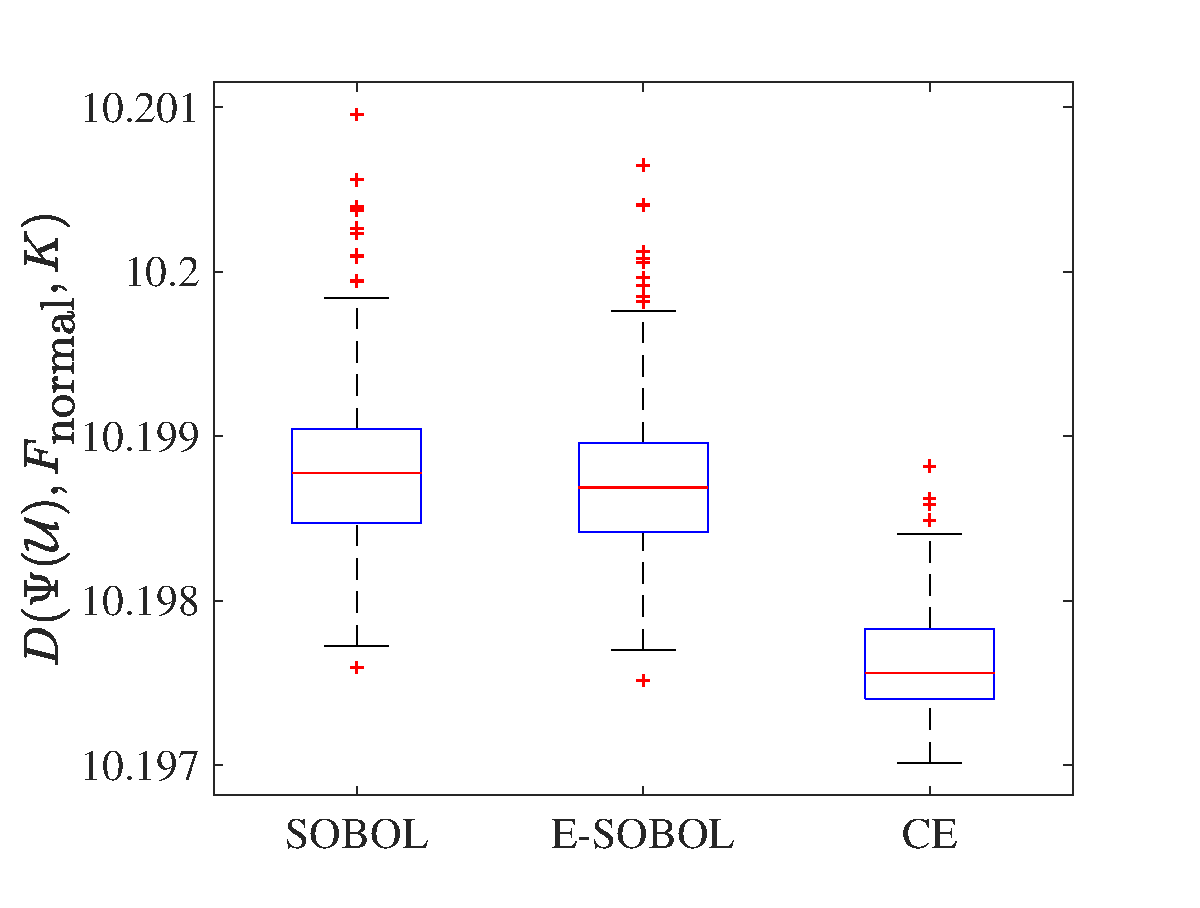
\includegraphics[width=5.5cm]{code/boxplot_d8n256.eps}}}
\quad
{\subfigure[$d=10, N=512$] {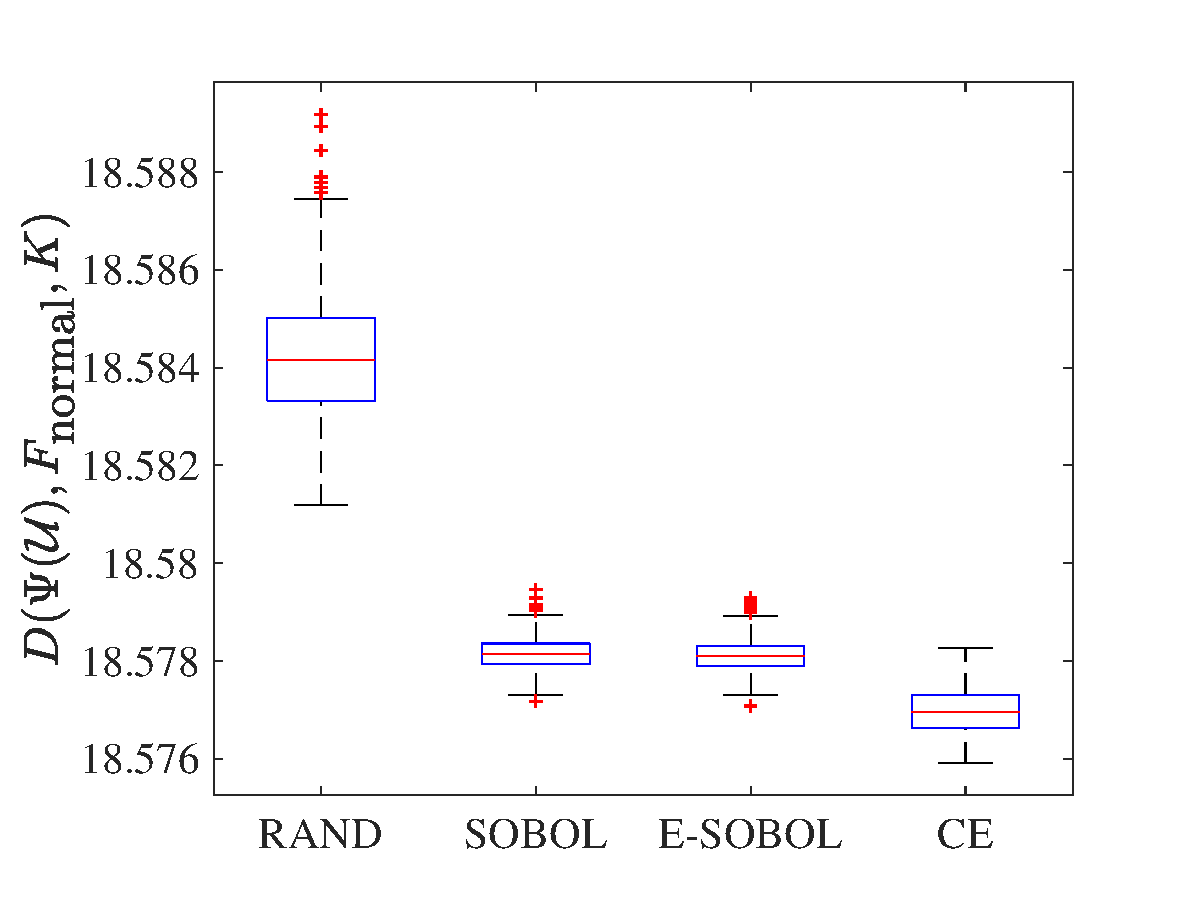
\includegraphics[width=5.5cm]{code/boxplotall_d10n512.eps}}}
\caption{Performance Comparison of Generators}
\end{figure}

We also report the average execution time of the four generators in Table \ref{tab:ExeTime}. All codes were run on a MacBook Pro with 2.4 GHz Intel Core i5 processor. Although CE requires the longest computational time compared to the other three generators, the execution time to achieve one sample is very reasonable. CE is quite computationally efficient and practical especially when the dimension is high and only a small sample is affordable.

% Table generated by Excel2LaTeX from sheet 'Sheet1'
\begin{table}[htbp]
  \centering
  \caption{Execution Time of Generators (in seconds)}
    \begin{tabular}{ccccccc}
    \hline
          & $d=2,$   & $d=3,$   & $d=4,$   & $d=6,$   & $d=8,$   & $d=10,$ \\
  & $N=32$   & $N=64$   & $N=64$   & $N=128$   & $N=256$   & $N =512$ \\
    \hline
    RAND  & $3.22\times 10^{-5}$      &  $5.21\times 10^{-5}$     & $5.27\times 10^{-5}$      &  $9.92\times 10^{-5}$     & $2.48\times 10^{-4}$      & $ 5.32\times 10^{-4}$ \\
    SOBOL & $8.60\times 10^{-4}$      &  $0.10\times 10^{-2}$     &    $0.11\times 10^{-2}$   &  $0.16\times 10^{-2}$     & $0.21\times 10^{-2}$      &  $0.28\times 10^{-2}$\\
    E-SOBOL & $8.71\times 10^{-4}$  & $0.11\times 10^{-2}$      &     $0.12\times 10^{-2}$  &  $0.16\times 10^{-2}$     &   $0.23\times 10^{-2}$    & $0.32\times 10^{-2}$  \\
    CE    & $1.34\times 10^{-2}$      & $2.73\times 10^{-2}$      & $6.12\times 10^{-2}$      &   $0.24$    &   $1.04$    & $3.84$  \\
    \hline
    \end{tabular}%
  \label{tab:ExeTime}%
\end{table}%

\begin{comment}
To further evaluate the performance of the normal random sequence generated by the four generators, we consider the integral approximation problem in \eqref{eq:badexample} with $d=10$. We use the Monte Carlo estimate with the sample generated by SOBOL of size $n = 2^{17}$ as an accurate estimate of the integral, and summarize the integral estimation error according to the four generators with simulation size $N=512$ in Figure \ref{fig:comparison_integral}. Not surprisingly, CE outperforms the other three generators and has no explosive relative error. It's interesting to see that SOBOL and E-SOBOL may perform even worse than RAND in several cases, and this aligns with our discussion in Section 4: the inverse transformed low uniform discrepancy sequence may not retain low normal discrepancy. When the sample size $N$ is small/moderate relative to dimension $d$, using CE would limit the potential danger of very inaccurate estimate caused by a sample with large normal discrepancy.



\begin{figure}[ht]\label{fig:comparison_integral}
\centering
{\subfigure[$d=2,N=32$] {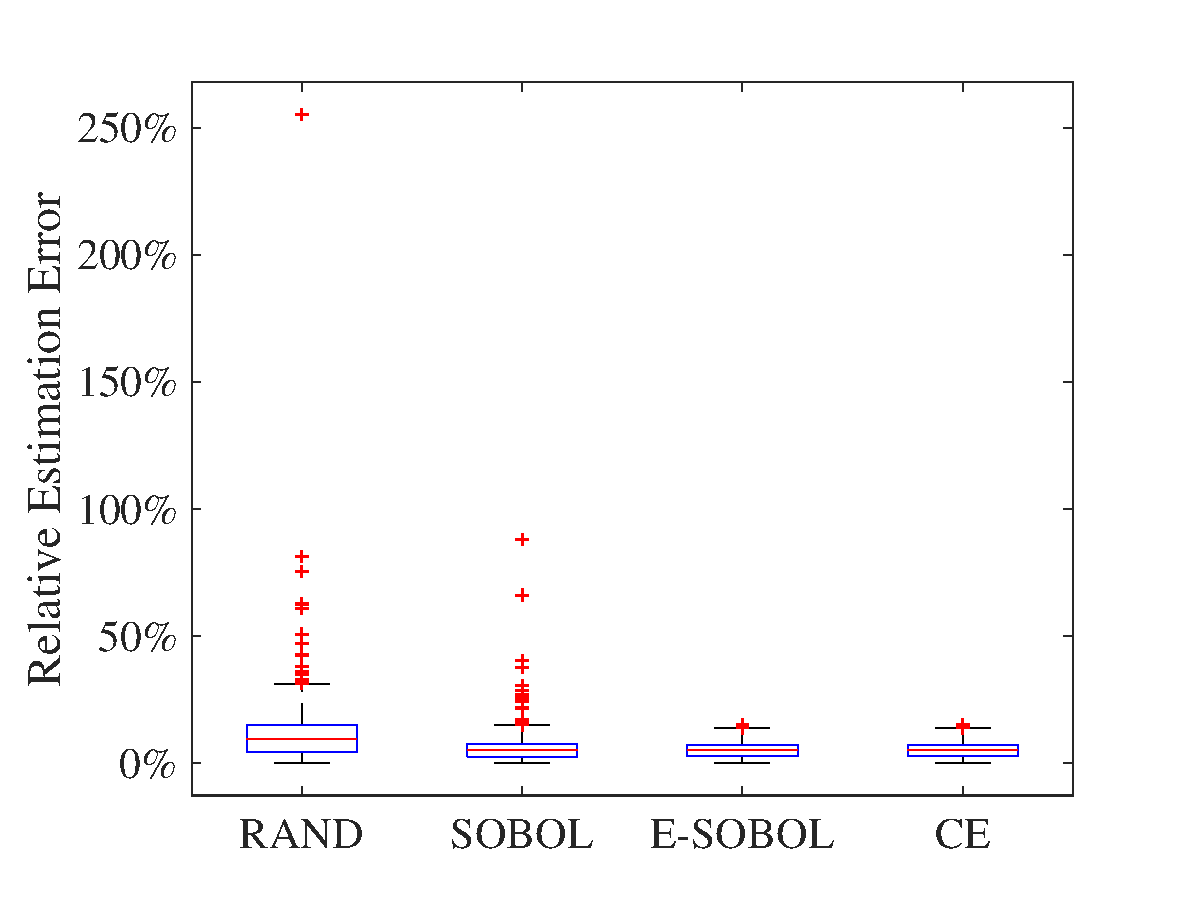
\includegraphics[width=5.5cm]{code/errorboxplot_d2n32.eps}}}
\quad
{\subfigure [$d=3, N=64$]
{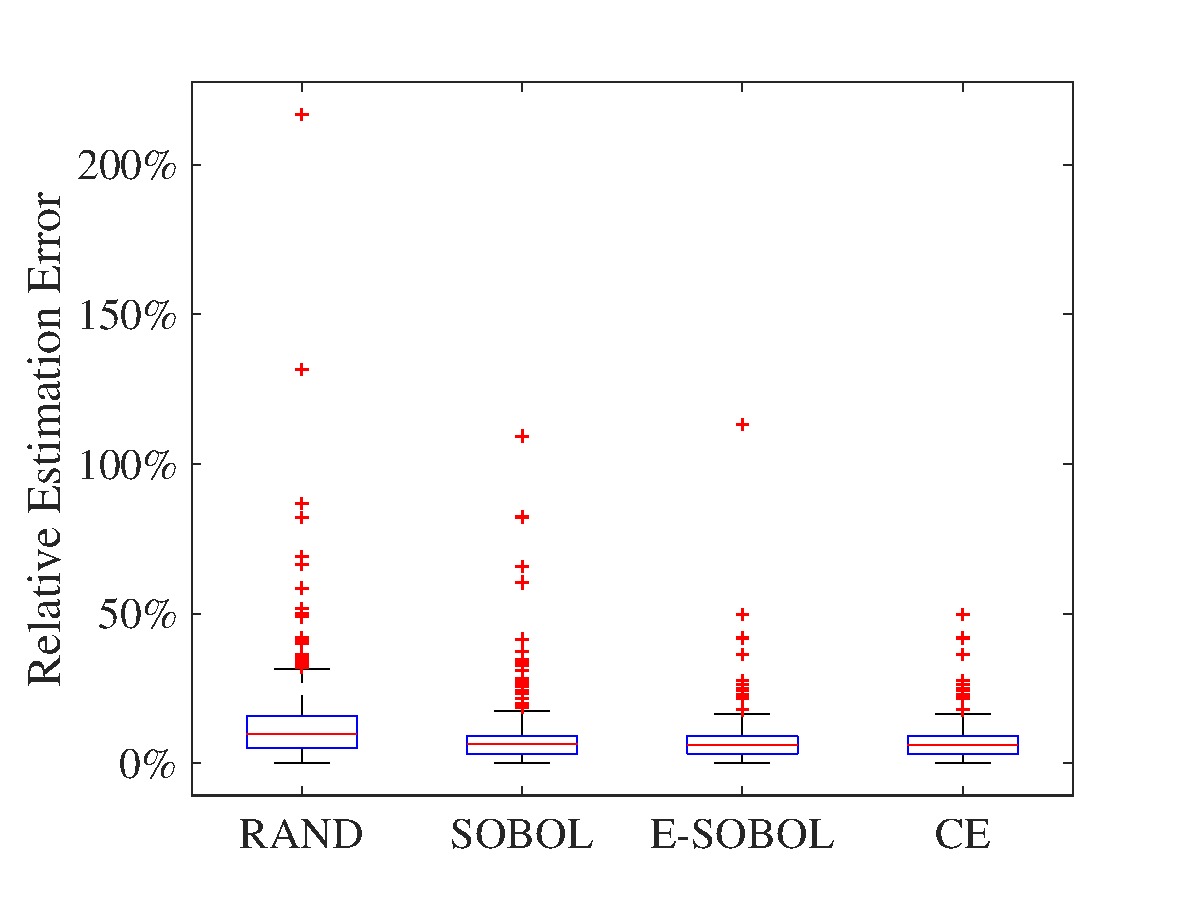
\includegraphics[width=5.5cm]{code/errorboxplot_d3n64.eps}}}
\quad
{\subfigure[$d=4, N=64$] {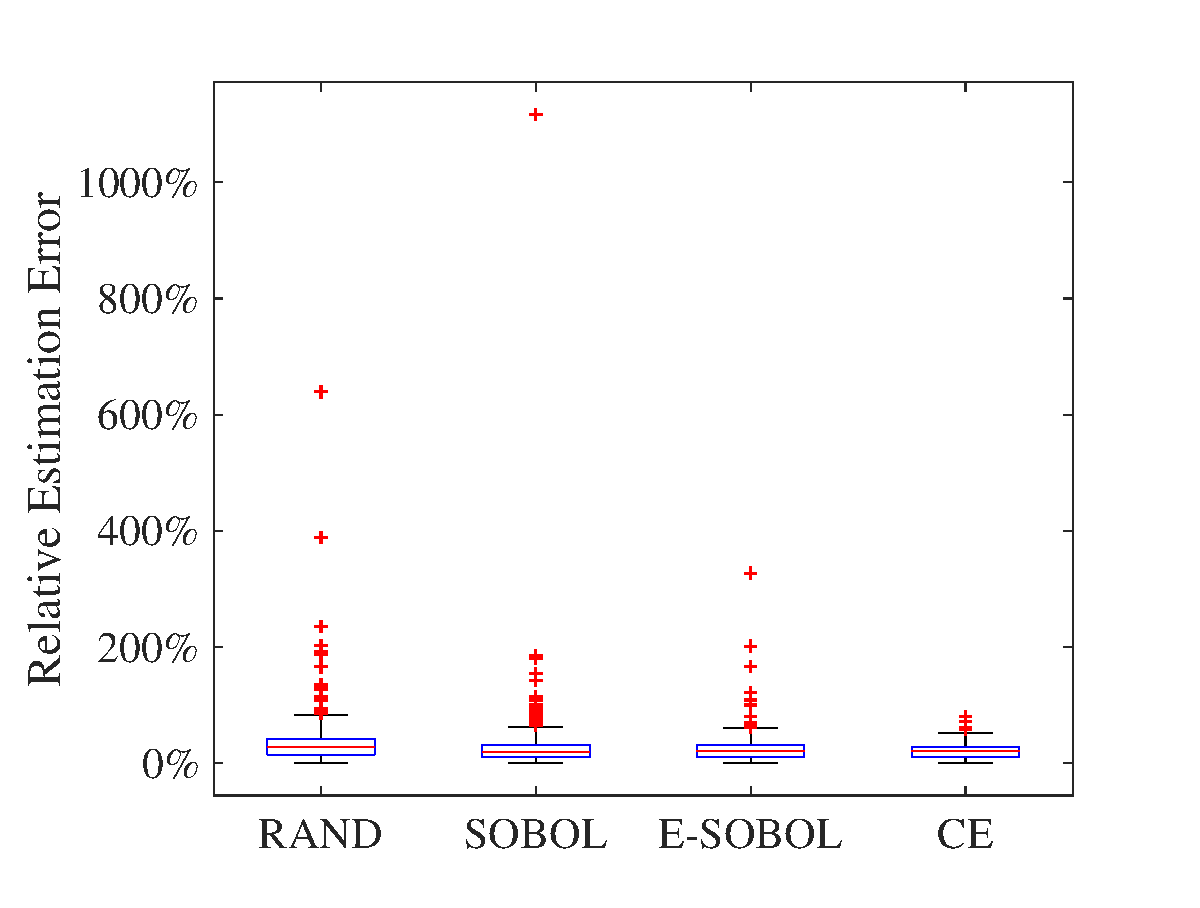
\includegraphics[width=5.5cm]{code/errorboxplot_d4n64.eps}}}
\quad
{\subfigure[$d=6, N=128$] {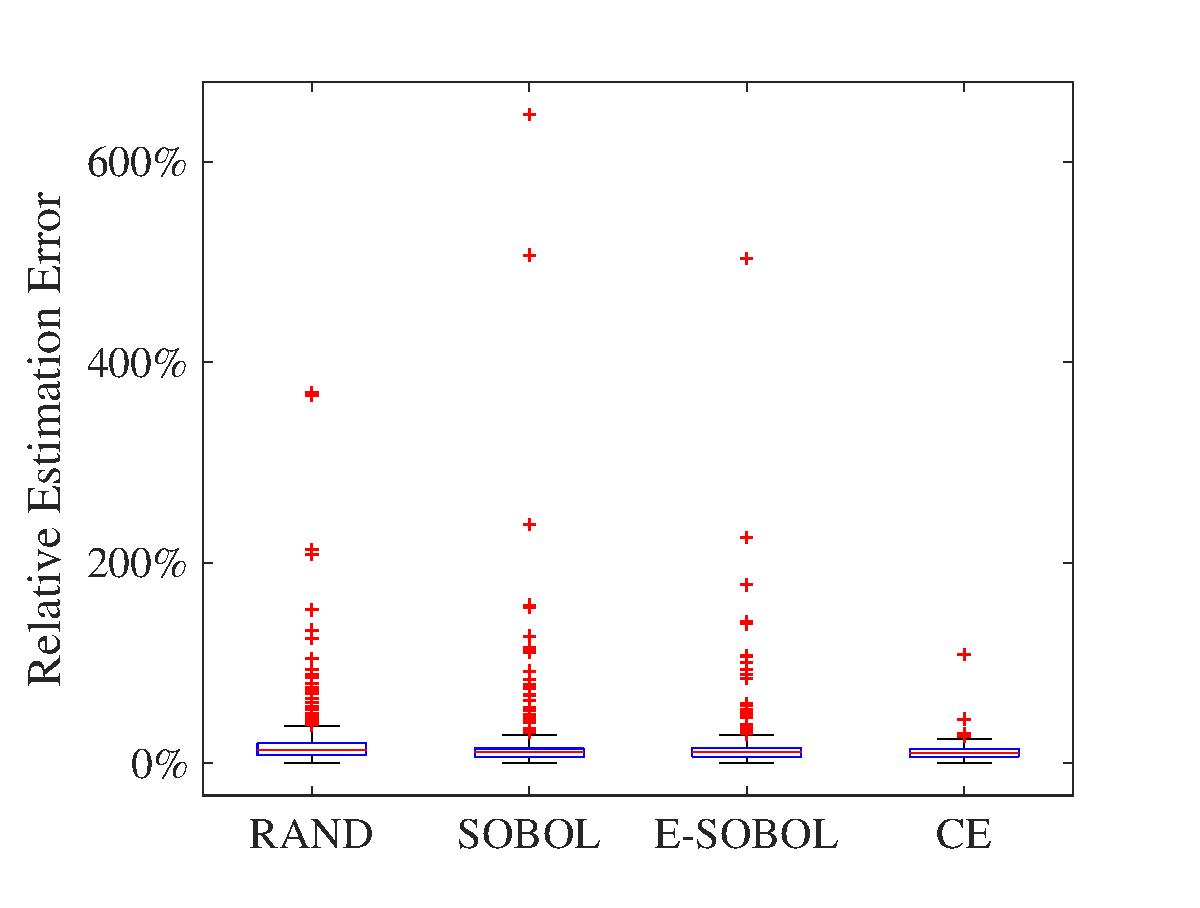
\includegraphics[width=5.5cm]{code/errorboxplot_d6n128.eps}}}
\quad
{\subfigure[$d=8, N=256$] {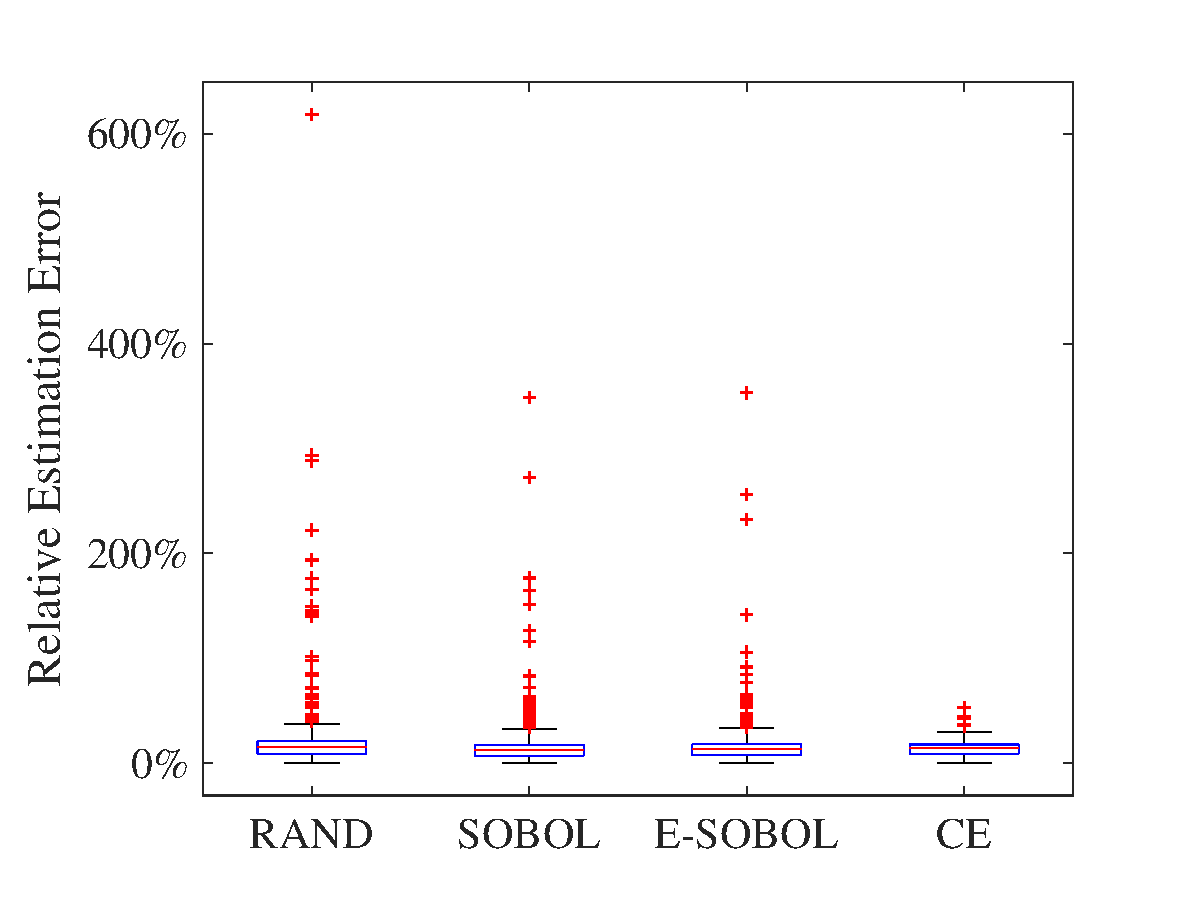
\includegraphics[width=5.5cm]{code/errorboxplot_d8n256.eps}}}
\quad
{\subfigure[$d=10, N=512$] {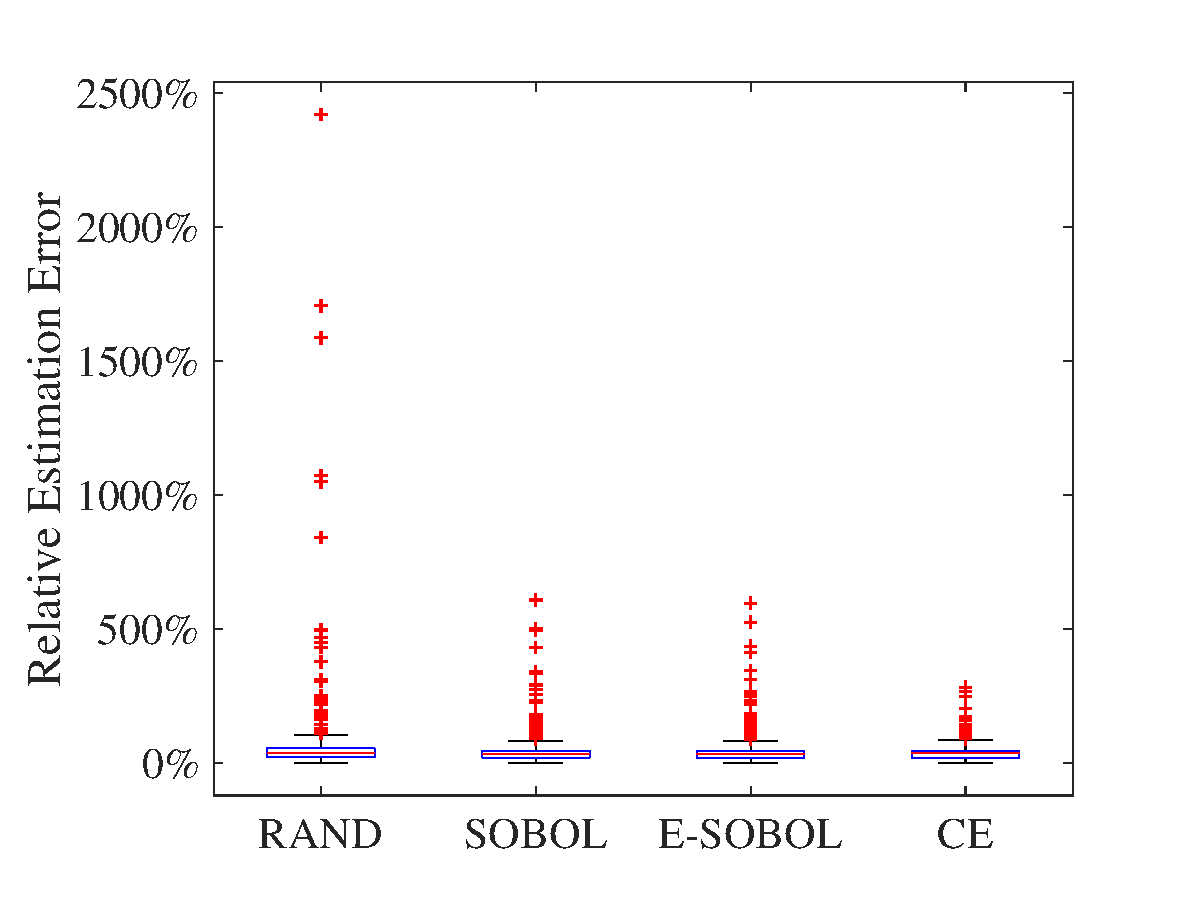
\includegraphics[width=5.5cm]{code/errorboxplot_d10n512.eps}}}
\caption{Integral Approximate Performance Comparison of Generators}
\end{figure}
\end{comment}



\section{Discussion}
In this chapter, we summarize the three interpretations of the discrepancy. 
It is a measure on how well the empirical distribution of a design approximates the target distribution or a tight upper bound of some quadrature of an integral approximation, or the root mean squared cubature error of an integral approximation when the integrand is a stochastic process. 
Then, we point out a flaw of the inverse transformation method, which is used to generate random samples (or designs) following any non-uniform distribution. 
The flaw is that any low-discrepancy uniform designs do not necessarily lead to low-discrepancy for the inverse transformed designs. 
To explain this issue, we choose the standard normal distribution as an example for non-uniform distributions. 
We show that the low-discrepancy uniform design may not preserve the low-discrepancy after inverse distribution transformation into a standard normal distribution. 
As a remedy approach, we propose a coordinate-exchange algorithm to further minimize the $L_2$-discrepancy of the design from the inverse transformation of the low-discrepancy uniform design. 

It's worth pointing out that the discrepancy defined in \eqref{eq:discDef} can be generalized to any $d$-dim distribution $\varrho$ with mean $\boldsymbol{\mu} = (\mu_1,\cdots,\mu_d)$. The centered reproducing kernel in \eqref{eq:OrigKernel} should be 
\begin{equation} \label{ExtKernel}
     K(\vt,\vx)  = \prod\limits_{j=1}^d\left[1+ \frac 12 \left(|t_j-\mu_j|+ |x_j-\mu_j|- |x_j-t_j| \right)\right].
\end{equation}
Then the discrepancy $D(\Xdes,\Ftar,K)$ can be computed using \eqref{eq:discDef}, and the two integrals in \eqref{eq:discDef} may require numerical approximations for some target distribution. 
If the analytic formula of $D(\Xdes,\Ftar,K)$ can be derived, the coordinate-exchange algorithms can be applied in a similar fashion to improve the inverse transformation method. 

\FJH{I should write about coordinate weights}


\section*{Appendix}
Derivation of \eqref{eq:DisNormald>1}. 
\begin{proof}
We first derive $D^2(\Xdes,\Phi_1,K)$ for $d=1$ case. 
To compute the discrepancy, we first integrate the kernel once:
\begin{align*}
\MoveEqLeft{\int_{-\infty}^\infty K(x,t) \, \dif \Phi_1(x)}\\
=&\int_{-\infty}^{\infty} \left(1+\frac{1}{2}|x|+\frac{1}{2}|t|-\frac{1}{2}|x-t|\right)\phi(x) \, \dif x\\
=& 1+ \frac{1}{\sqrt{2\pi}} + \frac{1}{2}|t|-\frac{1}{2}\left[\int_{-\infty}^{t}(t-x)\phi(x) \, \dif x+\int_{t}^{\infty} (x-t)\phi(x) \, \dif x\right]\\
=& 1+ \frac{1}{\sqrt{2\pi}} + \frac{1}{2}|t| - t [\Phi_1(t)-1/2] - \phi(t) .
\end{align*}
Then we integrate again:
\begin{align*}
\MoveEqLeft{\int_{-\infty}^\infty \int_{-\infty}^\infty K(x,t) \, \dif \Phi_1(x) \dif \Phi_1(t)}\\
& =  \int_{-\infty}^{\infty} \left( 1+\frac{1}{\sqrt{2\pi}} + \frac{1}{2}|t| - t [\Phi_1(t)-1/2] + \phi(t)\right)\phi(t) \, \dif t\\
&= 1+ \sqrt{\frac{2}{\pi}} + \int_{-\infty}^{\infty} \{ - t \Phi_1(t)\phi(t)  +  [\phi(t)]^2 \} \, \dif t\\
&= 1+\sqrt{\frac{2}{\pi}}-\frac{1}{\sqrt{4\pi}}+\int_{-\infty}^{\infty}\frac{1}{2\pi}e^{-t^2}\dif t\\
&= 1+\sqrt{\frac{2}{\pi}}-\frac{1}{\sqrt{4\pi}}+\frac{\frac{1}{\sqrt{2}}}{\sqrt{2\pi}}\int_{-\infty}^{\infty}\frac{1}{\sqrt{2\pi}\left(\frac{1}{\sqrt{2}}\right)}e^{-\frac{t^2}{2\left(\frac{1}{\sqrt{2}}\right)^2}}\dif t\\
&=1+\sqrt{\frac{2}{\pi}}. 
\end{align*}
Notice that $\int_{-\infty}^{\infty} t\Phi_1(t)\phi(t)\dif t = \frac{1}{\sqrt{4\pi}}$ and 
\begin{eqnarray*}
&&\int_{\Omega}K(x,x_n)\dif \Phi_1(x)\\
&=& \int_{-\infty}^{\infty} \left(1+\frac{1}{2}|x|+\frac{1}{2}|x_n|-\frac{1}{2}|x-x_n|\right)\phi(x)\dif x\\
&=& 1+\frac{1}{2}\sqrt{\frac{2}{\pi}}+\frac{1}{2}|x_n|-\frac{1}{2}\left[\int_{-\infty}^{x_n}(x_n-x)\phi(x)\dif x+\int_{x_n}^{\infty} (x-x_n)\phi(x)\dif x\right]\\
&=& 1+\sqrt{\frac{1}{2\pi}}+\frac{1}{2}|x_n|-\frac{1}{2}\left[\int_{-\infty}^{x_n}(x_n-x)\phi(x)\dif x+\int_{x_n}^{\infty} (x-x_n)\phi(x)\dif x\right]\\
&=& 1+\sqrt{\frac{1}{2\pi}}+\frac{1}{2}|x_n|-\frac{1}{2}\left[2x_n\Phi_1(x_n)-x_n-2\int_{-\infty}^{x_n}x\phi(x)\dif x\right]\\
&=& 1+\sqrt{\frac{1}{2\pi}}+\max(x_n,0)-x_n\Phi_1(x_n)-\frac{ e^{-x_n^2/2}}{\sqrt{2\pi}}. 
\end{eqnarray*}
Thus, the discrepancy can be obtained as follows. 
\begin{eqnarray*}
&& D^2(\Xdes,\Phi_1,K)=1+\sqrt{\frac{2}{\pi}}-\frac{2}{N}\sum_{n=1}^N \left[1+\sqrt{\frac{1}{2\pi}}+\max(x_n,0)-x_n\Phi_1(x_n)-\frac{ e^{-x_n^2/2}}{\sqrt{2\pi}}\right]\\
&&+\frac{1}{N^2}\sum_{n,m=1}^N \left[1+\frac{1}{2}|x_n|+\frac{1}{2}|x_m|-\frac{1}{2}|x_n-x_m|\right]\\
&= &-\frac{2}{N}\sum_{n=1}^N \left[\max(x_n,0)-x_n\Phi_1(x_n)-\frac{ e^{-x_n^2/2}}{\sqrt{2\pi}}\right]+\frac{1}{N^2}\sum_{n,m=1}^N \left[\frac{1}{2}|x_n|+\frac{1}{2}|x_m|-\frac{1}{2}|x_n-x_m|\right]\\
&=& -\frac{2}{N}\sum_{n=1}^N \left[\max(x_n,0)-x_n\Phi_1(x_n)-\phi(x_n)\right]+\frac{1}{N}\sum_{n=1}^N|x_n|-\frac{1}{2N^2}\sum_{n,m=1}^N|x_n-x_m|.\\
\end{eqnarray*}
For the distribution $N({\bf 0}, {\bf I}_d)$, the joint pdf is $$\prod\limits_{j=1}^d\phi(x_j) = \prod\limits_{j=1}^d \frac{1}{\sqrt{2\pi}}e^{-x_j^2/2}.$$
Here the cdf function $\Phi(\vx)=\prod_{j=1}^d \Phi_1(x_j)$. Thus, 
\begin{align*}
\int_{\reals^d\times \reals^d} K(\vx,\vt)&\dif\Phi(\vx)\dif\Phi(\vt) = \left(1+\sqrt{\frac{2}{\pi}}\right)^d, \\
\int_{\reals^d}K(\vx,\vx_n)\dif\Phi(\vx) = \prod\limits_{j=1}^d&\left[ 1+\frac{1}{\sqrt{2\pi}}+\frac{1}{2}|x_j|-x_j[\Phi(x_j)-1/2]-\phi(x_j)\right].
\end{align*}
The discrepancy can be obtained
\begin{eqnarray*}
&&D^2(\Xdes, \Phi, K)\\
&=& \left(1+\sqrt{\frac{2}{\pi}}\right)^d - \frac{2}{N}\sum\limits_{\vx\in P} \prod\limits_{j=1}^d\left[ 1+\frac{1}{\sqrt{2\pi}}+\frac{1}{2}|x_j|-x_j[\Phi_1(x_j)-1/2]-\phi(x_j)\right]\\
&&+\frac{1}{N^2}\sum_{\vx,\vt\in P}\prod_{j=1}^d \left[1+\frac{1}{2}|x_j|+\frac{1}{2}|t_j|-\frac{1}{2}|x_j-t_j|\right]. 
\end{eqnarray*}       
\end{proof}

\bibliographystyle{amsplain}
%\bibliography{FJH23,FJHown23}
\bibliography{Ref.bib,FJH23,FJHown23}

\end{document}


